%****************************************************
%	CHAPTER 2 - Prototype Design
%****************************************************
\chapter{Prototype Design}
\label{ch:proto}
%====================================================
\section{Design}
\label{sec:proto.design}
%====================================================
\begin{figure}[htbp]
\centering
%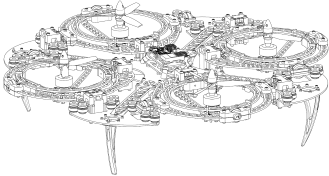
\includegraphics[width=0.93\textwidth]{figs/iso-design}
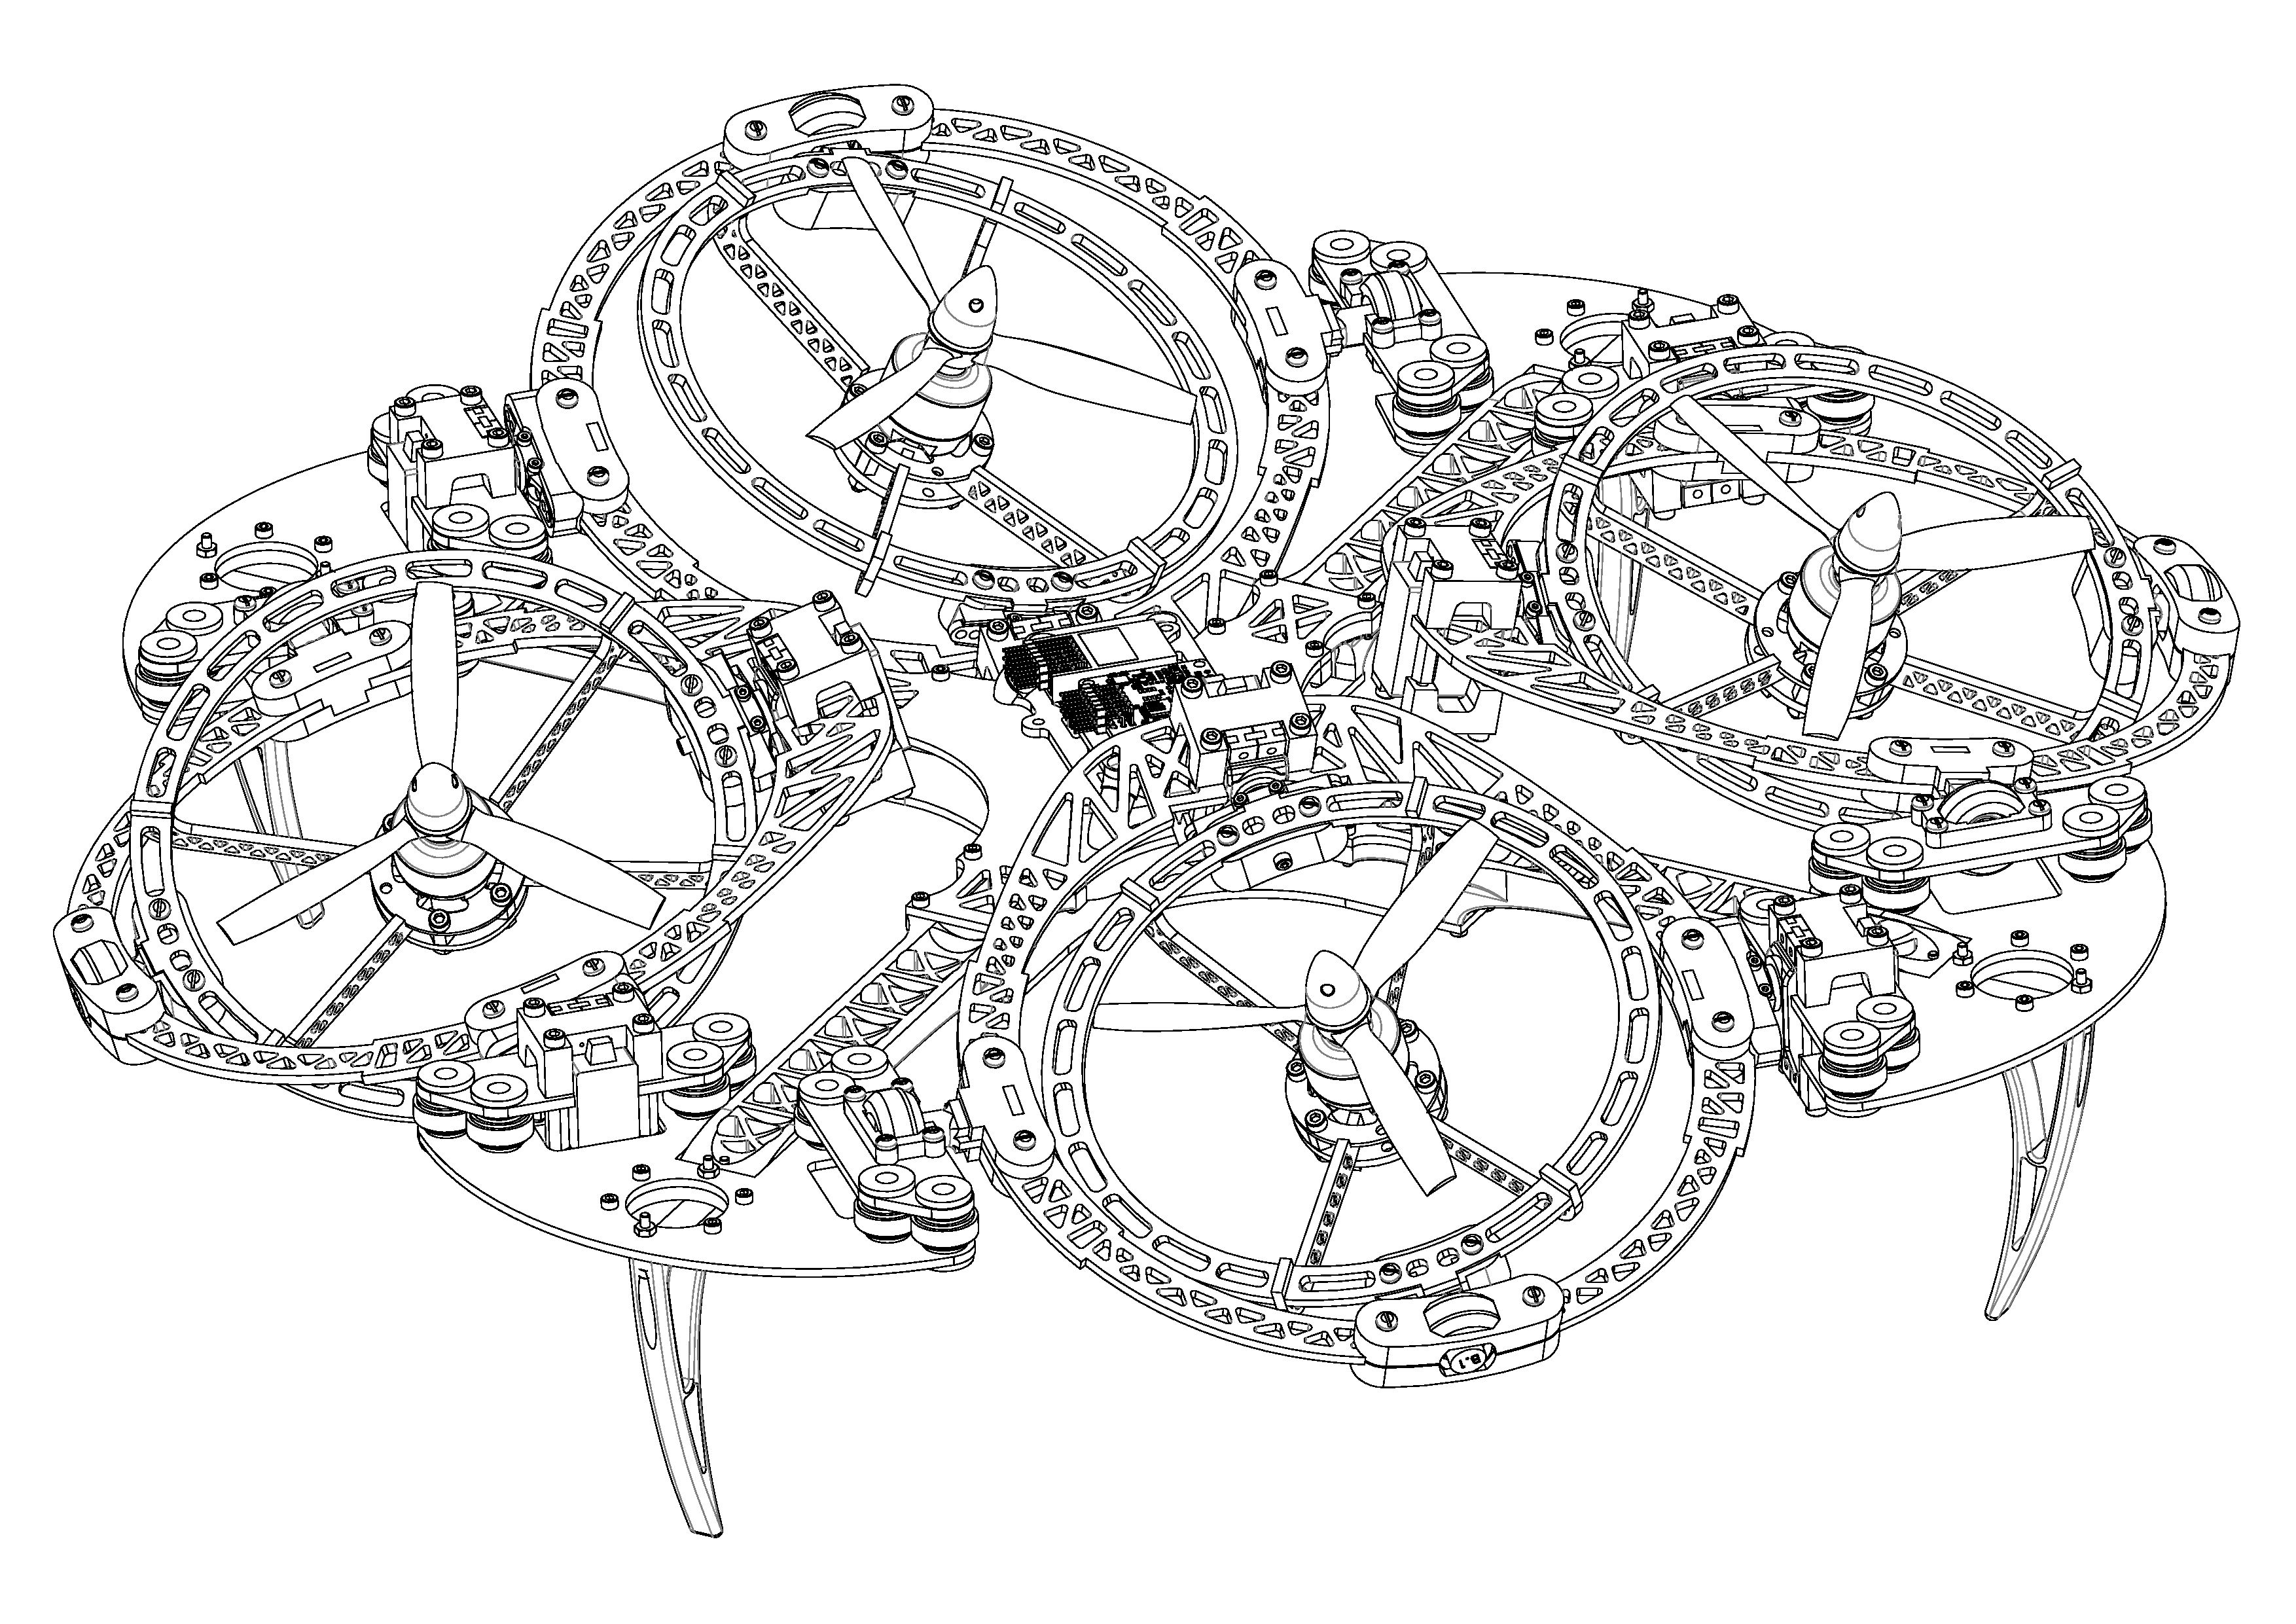
\includegraphics[width=\textwidth]{pdfpages/iso-design.pdf}
\vspace{-34pt}
\caption{Isometric view of the prototype design}
\vspace{-4pt}
\label{fig:iso-design}
\end{figure}
\par
The final prototype (Fig:\ref{fig:iso-design}) went through a series of different design iterations, aimed at optimizing engineering time spent on construction and reducing the associated component costs. Significant consideration for the design process was the net weight whose upper limit is inherently limited by the thrust produced from lift motors. Some of the more important design factors, like inertial matrices and associated masses (Sec:\ref{sec:proto.inertia}), are discussed here in order to give context for the dynamics derived later in Ch:\ref{ch:dynamics}. The reference frame orientations (which those dynamics are developed with respect to) are detailed here. A brief overview of the electrical systems layout is then given with the components associated and their electrical characteristics included. Finally the actuator suite's functionality and transfer characteristics are quantified.
%====================================================
\subsection{Actuation Functionality}
\label{subsec:proto.design.actuation}
%====================================================
The most important component of the design is the articulation for each of the four vectored thrust forces. A concentric gimbal ring structure (Fig:\ref{fig:motor-assembly}) independently redirects each lift propeller/motor about two separate rotational axes. Within each module are servos affixed onto sequential gyroscope-like support rings to accommodate pitching and rolling of the propeller's direction. Aligned with each servo is a coaxial support bearing. The bearing and actuator servos have a mass disparity which results in an eccentric center of mass, producing a net gravitational torque arm. Unfortunately, due to weight constraints, counter balance measures cannot be introduced. Consequences from the center of mass variations must be either compensated for (\emph{plant dependent solution}) or exploited in the dynamics (\emph{additional nonlinear actuator plants}). The precise effects are quantified numerically later in Sec:\ref{sec:proto.inertia}.
\par
\begin{figure}[hbtp]
\begin{subfigure}{.49\textwidth}
\centering
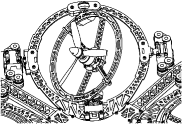
\includegraphics[width=\textwidth]{figs/motor-assembly}
\caption{Motor module assembly}
\label{fig:motor-assembly}
\end{subfigure}
\begin{subfigure}{.49\textwidth}
\centering
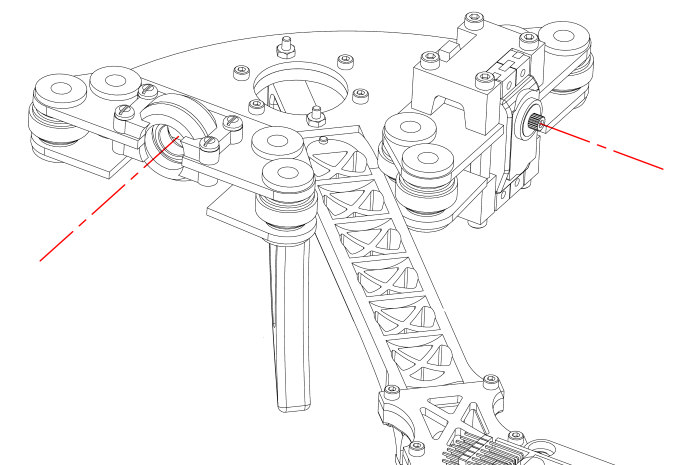
\includegraphics[width=\textwidth]{figs/motor-support}
\caption{Motor frame damping support assemblies}
\label{fig:motor_support}
\end{subfigure}
\caption{Tilting rotor design}
\end{figure}
Each motor module is positioned such that its produced thrust vector coincides with the intersection of its two rotational axes (Fig:\ref{fig:motor-assembly}). As a result there is only a perpendicular displacement of the thrust vector, $L_{arm}=195.16~\text{mm}$, co-planar to the body frame's X-Y-Z origin $\vec{\mathbf{O}}_b$ (see subsequent Fig:\ref{fig:motor-frame}). That length directly affects the differential torque plant; $\vec{\tau}_{diff}=\sum\vec{L}_i\times\vec{T}_i$. An eccentric thrust vector line would make the torque arm displacement a non-orthogonal vector. The center of gravity for each module is time varying and depends on the two servo rotational positions. It is more prudent to ensure intersection of the thrust vector with the rotational center than to balance the masses undergoing rotation. A thrust varying torque is harder to approximate and hence compensate for than a gravitational torque, given the complexity of modeling a propeller's aerodynamic thrust (Sec:\ref{subsec:dynamics.aero.bem}).
\par
The primary body structure is similar to a traditional quadcopter `+' configuration with adjacent propellers spinning in opposite directions. Each motor module's rotational assembly is suspended by silicone damping balls (Fig:\ref{fig:motor_support}). A smaller damping assembly in the center of the frame houses all the electronics and power distribution circuitry. All the mounting brackets affixing the motor module rings are 3D printed from CAD models using an Ultimaker V2+\cite{ultimaker}. A complete bill of materials for all parts used, including working drawings for each 3D printed bracket and the laser cut frame(s), is presented in App:\ref{app:bom}.
\par
\begin{figure}[hbtp]
\centering
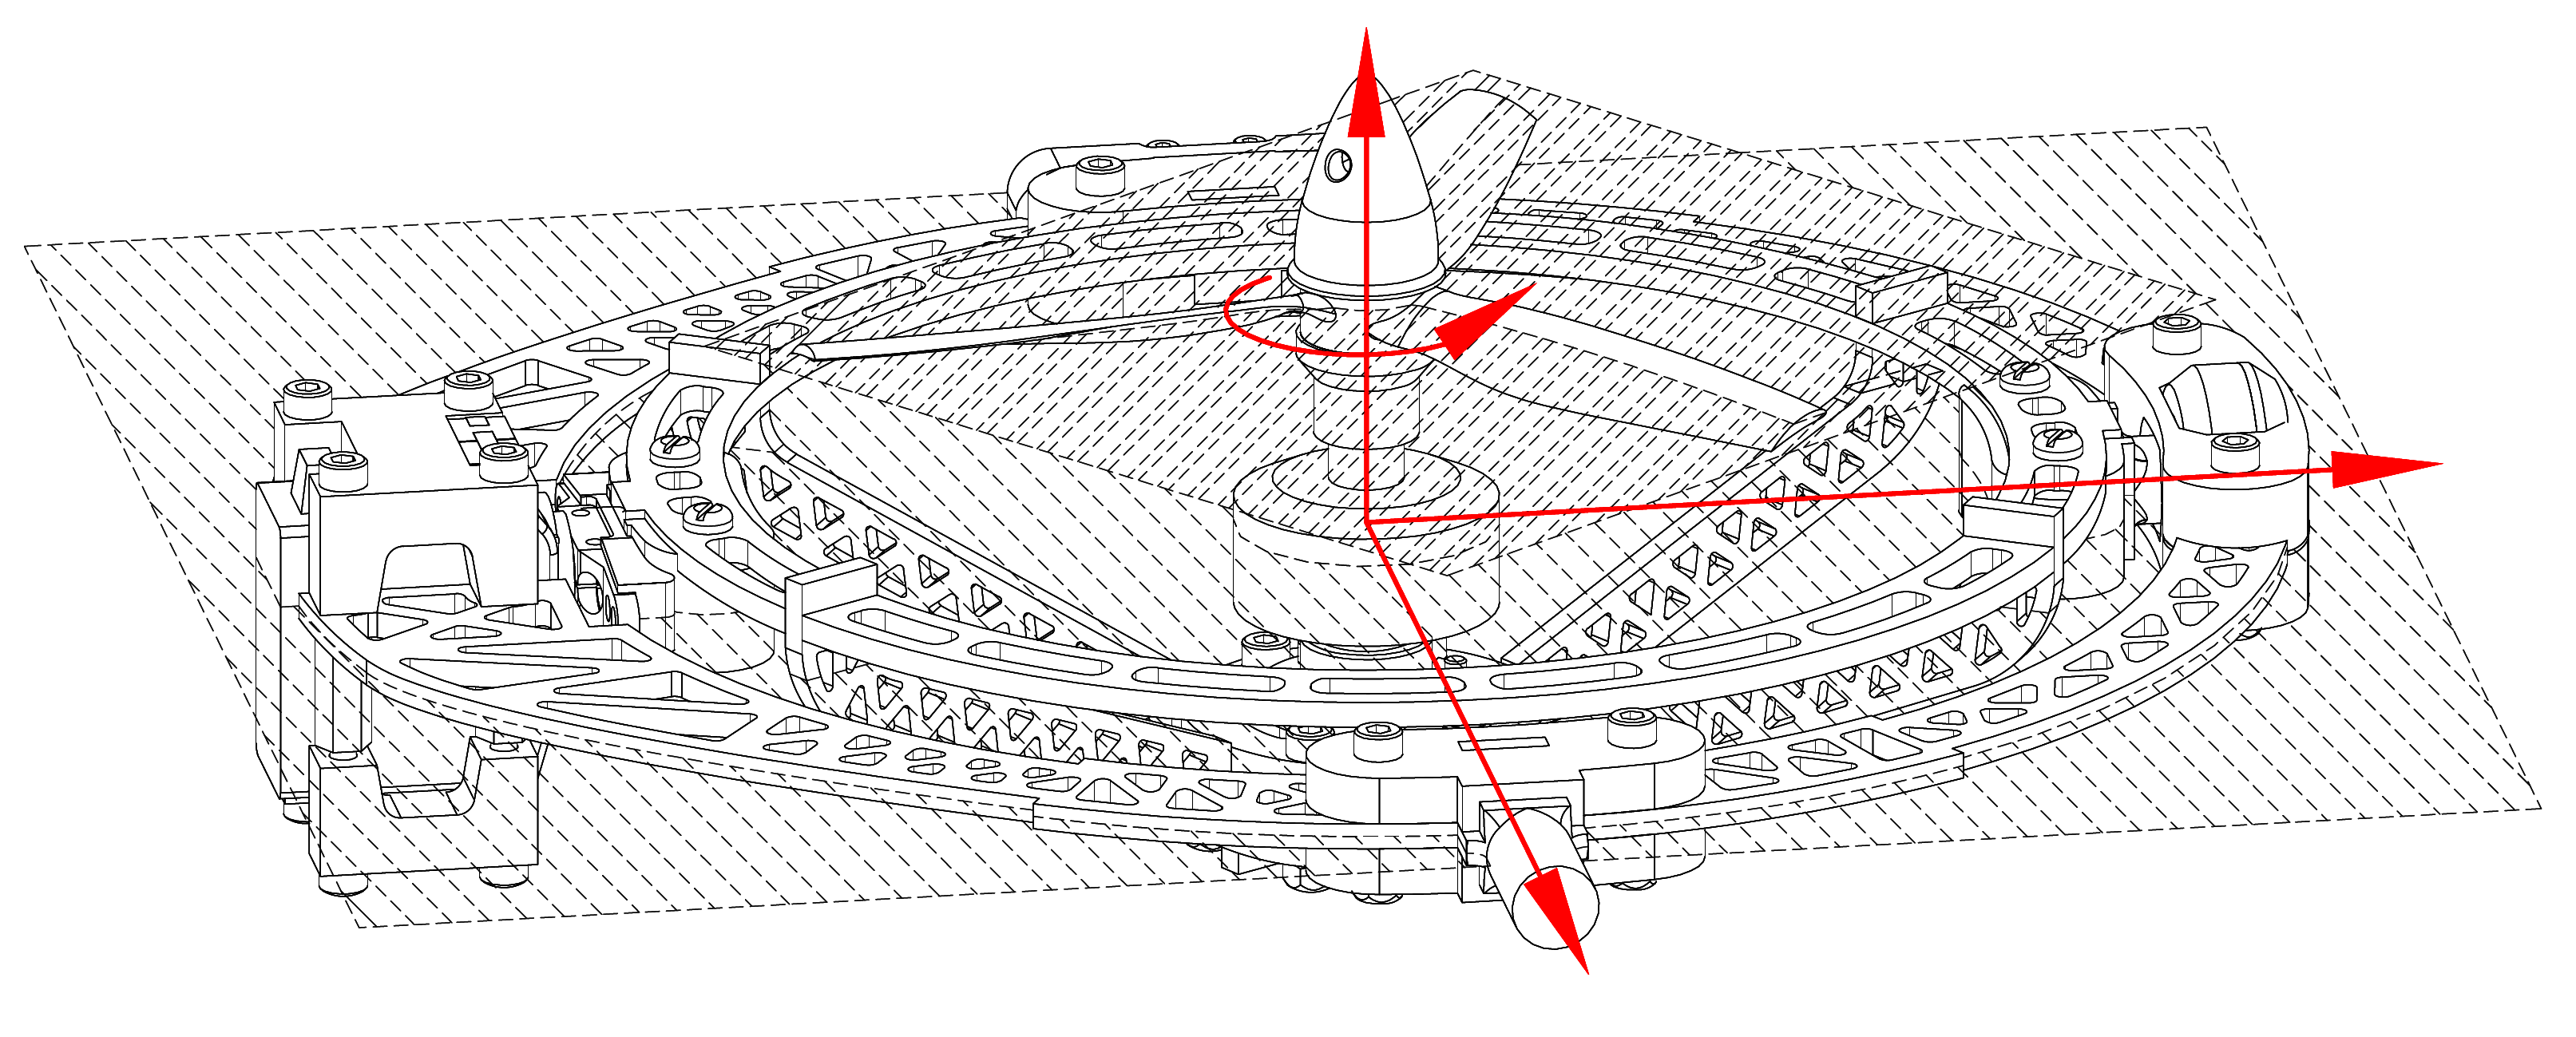
\includegraphics[width=0.85\textwidth]{figs/motor-prop}
\vspace{-10pt}
\caption{Difference between propeller and motor planes}
\label{fig:motor_prop}
\vspace{-15pt}
\end{figure}
The propeller's rotational plane is not aligned exactly with the plane made by the $\hat{X}_{M_i}$ and $\hat{Y}_{M_i}$ rotational servo axes (Fig:\ref{fig:motor_prop}). The offset is approximately $23.0~\text{mm}$ and must be considered when evaluating pitch/roll inertial and gyroscopic torque responses later in Sec:\ref{subsec:dynamics.nonlinearities.gyrotorques}. The propellers are six inch ($6 \times 4.5$) three-bladed plastic Gemfam propellers, powered by Cobra CM2208-2000 KV Brushless DC motors (Fig:\ref{fig:bldc-motor}). The thrust produced as a function of angular velocity (in revolutions per second) for the propellers is derived in Sec:\ref{subsec:dynamics.aero.bem}. 
\newpage
The BLDC motors are controlled with LDPower 20A ESC modules with an in-line OrangeRx RPM Sensor. The ESCs were reflashed with BLHeli\cite{BLHeli} firmware. The default firmware on the speed controllers had an unsatisfactory exponentially approaching, nonlinear input speed curve; in contrast with the linear unloaded speed curve in Fig:\ref{fig:rpm-sensor}. The net transfer functions for both ESC modules and the servos are detailed later in Sec:\ref{subsec:proto.design.transfer}. Power for the quadrotor is supplied from a power tether (not from a battery bank). Tethered power will ensure consistent flight time and reduce the concern of payload restriction on the available lift actuation. Power lines to both the BLDC motors and servos are supplied through conventional wiring, however an ideal and more flexible design would see slip-rings for each module's power supply. 
\begin{figure}[htbp]
\centering
\begin{subfigure}{0.49\textwidth}
\centering
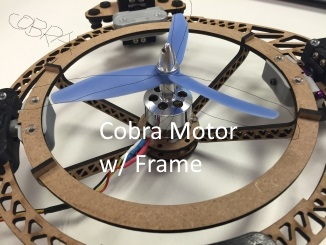
\includegraphics[width=0.9\textwidth]{figs/motor-bldc}
\caption{Cobra CM2208-2000KV BLDC motor module}
\label{fig:bldc-motor}
\end{subfigure}
\begin{subfigure}{0.49\textwidth}
\centering
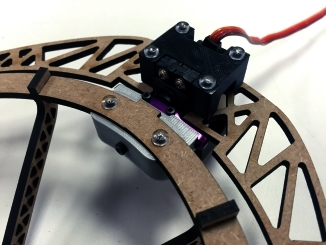
\includegraphics[width=0.9\textwidth]{figs/motor-servo}
\caption{Corona DS-339MG servo bracket}
\label{fig:motor-servo}
\end{subfigure}
\vspace{-5pt}
\caption{Motor module assembly}
\vspace{-15pt}
\end{figure}
\par
Metal gear Corona DS-339MG digital servos are used for the two axes of rotation (Fig:\ref{fig:motor-servo}). Each servo has a rotational range of $\approx 180\text{\textdegree}$, positioned such that a $\text{zero}^{\text{th}}$ offset aligns the motor modules, adjacent to the body frame, and has a $\pm 90\text{\textdegree}$ rotational range. A digital servo updates at 330 Hz, faster than a 50 Hz analogue servo equivalent (Fig:\ref{fig:servo-timing}). This means the otherwise $20~\text{ms}$ zero-order ``analogue" sampling effect is a less significant $3.30~\text{ms}$ zero-order holding time. Both the $\hat{X}_{M_i}$ and $\hat{Y}_{M_i}$ axis servos will be rotating differing inertial bodies; as such their open loop transfer functions are individually determined through testing in Sec:\ref{subsec:proto.design.transfer}.
\begin{figure}
\centering
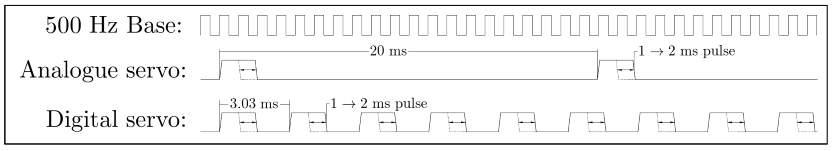
\includegraphics[width=0.75\textwidth]{figs/servo-timing}
\caption{Digital and analogue servo timing}
\label{fig:servo-timing}
\vspace{-20pt}
\end{figure}
%====================================================
\section{Reference Frames Used}
\label{sec:proto.conventions}
Attitude conventions used for deriving the system's dynamics in Ch:\ref{ch:dynamics}~are first discussed here. Often these aspects are assumed to be obvious enough that they are omitted. It is important to clearly and unambiguously define a standard set of framing conventions to avoid uncertainty later. Rotation matrices are included but the focus is on the \emph{contrast} between rotation and transformation operations. Both \cite{spacecraftattitutdequaternions} and \cite{rigidbodylecture} provide an in-depth and thorough explanation of rotation matrices and direct cosine matrix attitude representation, if such concepts are unfamiliar to the reader. Later quaternions are used to replace rotation matrix notation for the dynamics in Sec:\ref{subsec:dynamics.rigidbody.quaternion}.
%====================================================
\subsection{Reference Frames Convention}
\label{subsec:proto.conventions.frames}
%====================================================
\begin{figure}[htbp]
\centering
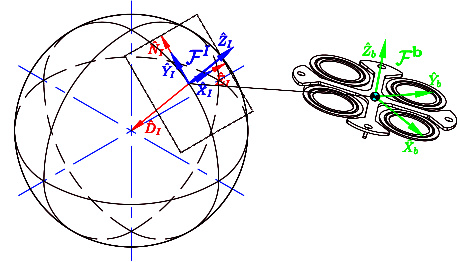
\includegraphics[width=0.8\textwidth]{figs/reference-frame}
\caption{Inertial and body reference frames}
\label{fig:ref_frame}
\end{figure}
NASA aerospace frames are used for principle Cartesian inertial and body coordinate representation (Fig:\ref{fig:ref_frame}). The inertial frame,~$\mathcal{F}^I$ with an origin $\vec{\mathbf{O}}_I$, is aligned such that the $\hat{Y}_I$ axis is in the $\hat{N}$orth direction, $\hat{X}_I$ is in the $\hat{E}$ast direction and $-\hat{Z}_I$ is  in the $\hat{D}$ownward direction. In Euler orbital sequences the $\hat{Z}$ direction would be toward the Earth's center, sometimes referred to as the N\^{E}D convention which differs from the NASA frames used here. The body frame, $\mathcal{F}^b$ centered on the point $\vec{\mathbf{O}}_b$, then has both $\hat{X}_b$ and $\hat{Y}_b$ aligned obliquely between two perpendicular arms of the quadrotor's body and the $\hat{Z}_b$ axis in the body's normal upward direction (illustrated in Fig:\ref{fig:body-frame}). 
\par
The body frame's axes and center of motion relative to the prototype design's center of mass are both detailed next in Sec:\ref{subsec:proto.conventions.motoraxis}. Frame superscripts $I$ and $b$ represent inertial and body frames respectively whilst vector subscripts imply the reference frame in which the vector's coordinates exists or taken relative to. The function $R_I^b(\eta)$ represents a rotation operator of the Euler set $\vec{\eta}$ (expanded on in Eq:\ref{eq:inertialbodytransformation}) rotating from subscript frame $\mathcal{F}^I$ to superscript frame $\mathcal{F}^b$. 
\par
A vector $\vec{\nu}$ has the relationship between the body and inertial frames:
\begin{equation}
\vec{\nu}_I=R_b^I(\eta)\vec{\nu}_b~~~~~~\vec{\nu}_b\in\mathcal{F}^b,~\vec{\nu}_I\in\mathcal{F}^I
\end{equation}
Displacement between the inertial and body frames is given by $\vec{\mathcal{E}}_I$ defined in the inertial frame:
\begin{equation}\label{eq:position-frame}
\vec{\mathcal{E}}_I=\begin{bmatrix}
x & y & z\end{bmatrix}^T~~~~\in\mathcal{F}^I
\end{equation}
An axial hat and upper case differentiates axis unit vectors $\hat{X},\hat{Y},\hat{Z}$ from inertial position quantities $x,y,z$ in Eq:\ref{eq:position-frame}. The body position's time derivative $\dot{\vec{\mathcal{E}}}_I$ refers to the \emph{inertial frame} rate:
\begin{equation}
\frac{d}{dt}\vec{\mathcal{E}}_I=\begin{bmatrix}
\dot{x} & \dot{y} & \dot{z}\end{bmatrix}^T~~~~\in\mathcal{F}^I
\end{equation}
Whereas the body's translational velocity $\vec{v}_b$ is with respect to the body frame $\mathcal{F}^b$. Velocity and the inertial position time derivative are related as follows:
\begin{subequations}
\begin{equation}
\vec{v}_b=R_I^b(\eta)\dot{\vec{\mathcal{E}}}_I~~~~\in\mathcal{F}^b
\end{equation}
\vspace{-18pt}
\begin{equation}
=R_I^b(\eta)\begin{bmatrix}
\dot{x} & \dot{y} & \dot{z}
\end{bmatrix}^T~~~~
\end{equation}
\end{subequations}
Relative angular displacement between two frames is commonly measured by the three angle Euler set. The Euler angle set $\vec{\eta}=[\phi ~\theta ~\psi]^T$ represents pitch $\phi$, roll $\theta$ and yaw $\psi$ rotations about sequential $\hat{X}$,$\hat{Y}$ and $\hat{Z}$ axes respectively. Depending on how the rotation sequence is formulated, those angles can be used to construct rotation matrices which give relation to vectors or can transform coordinates. 
\par
The general rotation equation to \emph{rotate} some vector $\vec{\nu}$ about a normalized unit axis $\hat{u}$ through a rotation angle $\theta$ is given by the rotation formula, derivated in \cite{rigidbodymotion}:
\begin{equation}\label{eq:genrotationmatrix}
\vec{\nu}~'=\big(1-cos(\theta)\big)\big(\vec{\nu}\cdot \hat{u}\big)\hat{u}+cos(\theta)\vec{\nu}+sin(\theta)\big(\hat{u}\times\vec{\nu}\big)
\end{equation}
In Eq:\ref{eq:genrotationmatrix}, when the unit vector $\hat{u}$ is in the direction of either $\hat{X}$; $\hat{Y}$ or $\hat{Z}$ axes the equation is simplified to produce the three fundamental rotation matrices $R_x(\phi)$; $R_y(\theta)$ and $R_z(\psi)$. That set of three principle rotation matrices about the Cartesian X-Y-Z axes are defined as:
\begin{subequations}\label{eq:rotationmatrix}
\begin{equation}
R_x(\phi)=\begin{bmatrix}
1 & 0 & 0\\
0 & cos(\phi) & -sin(\phi)\\
0 & sin(\phi) & cos(\phi)
\end{bmatrix}
\end{equation}
\vspace{-2pt}
\begin{equation}
R_y(\theta)=\begin{bmatrix}
cos(\theta) & 0 & sin(\theta)\\
0 & 1 & 0\\
-sin(\theta) & 0 & cos(\theta)
\end{bmatrix}
\end{equation}
\begin{equation}
R_z(\psi)=\begin{bmatrix}
cos(\psi) & -sin(\psi) & 0\\
sin(\psi) & cos(\psi) & 0\\
0 & 0 & 1
\end{bmatrix}
\end{equation}
\end{subequations}
The notation for a rotation matrix operation is multiplication of the matrix $R_{u}(\theta)$, applying a left-handed \emph{rotation} operator about some axis $\hat{u}$ by $\theta$. The resultant vector of a rotation operation still exists in the same reference frame. For example an $\hat{X}$ axis rotation by $\phi$ of some vector $\vec{\nu}$ is given by:
\begin{subequations} \label{eq:rotationoperator}
\begin{equation}\label{eq:rotationoperator.a}
\vec{\nu}^{\hspace{1pt}}\text{}'=R_{x}(\phi)\vec{\nu}~~~~~\vec{\nu}^{\hspace{2pt}}\text{}',\vec{\nu}\in\mathcal{F}^1
\end{equation}
\end{subequations}
No subscripts are used in Eq:\ref{eq:rotationoperator} to indicate reference frame ownership because all vectors are in the same frame. The time derivative of a rotation matrix about some axis $\hat{u}$ by a rotation $\theta$, $\dot{R}_u(\theta)$ is shown in \cite{quaddynamics} to be:
\begin{subequations}\label{eq:rotation-matrix-derivative}
\begin{equation}
\frac{d}{dt}\big(R_u(\theta)\big)=\big(\dot{\theta}\cdot\hat{u}\big)\times R_u\Rightarrow\big[\dot{\theta}\cdot\hat{u}\big]_{\times}R_u
\end{equation}
Where $\dot{\theta}\cdot\hat{u}$ is the projection of the angular rate $\dot{\theta}$ onto the $\hat{u}$ axis. Furthermore, for some vector $\vec{a}$, the operator $[\vec{a}\hspace{1pt}]_\times$ denotes the cross-product matrix or \emph{skew} matrix. The symmetric skew matrix is a matrix multiplication to replace the cross-product operator, for some other vector $\vec{b}$;
\begin{equation}
\vec{a}\times\vec{b}\equiv\big[\vec{a}\hspace{1pt}\big]_\times\vec{b}
\end{equation}
\vspace{-12pt}
\begin{equation}\label{eq:cross-product-matrix}
\rightarrow\big[\vec{a}\big]_\times\triangleq\begin{bmatrix}
0 & -a_3 & a_2\\
a_3 & 0 & -a_1\\
-a_2 & a_1 & 0
\end{bmatrix}
\end{equation}
\end{subequations}
A vector \emph{transformation} changes the resultant vector's reference frame. The transformation is then a rotation by an angle of the \emph{difference} (or negative angle) between the resulting and principle reference frames. A transformation from frame $\mathcal{F}^1$ to $\mathcal{F}^2$, differing by an angle of $\phi$ about the $\hat{X}$ axis is then a negative rotation operation:
\begin{subequations}\label{eq:transformationoperator}
\begin{equation}\label{eq:transformationoperator.a}
\vec{\nu}_2=R_x(-\phi)\vec{\nu}_1
\end{equation}
\vspace{-15pt}
\begin{equation}\label{eq:transformationoperator.b}
\vec{\nu}_2\in\mathcal{F}^2~\text{and}~\vec{\nu}_1\in\mathcal{F}^1
\end{equation}
\end{subequations}
The distinction between Eq:\ref{eq:rotationoperator} and Eq:\ref{eq:transformationoperator} is the directional sense of the angular operand $\phi$, and hence the effect it has on the argument vector. The transformation or rotation of a vector from the inertial frame $\mathcal{F}^I$ to the body frame $\mathcal{F}^b$ is the product of three sequential operations about each princple axis. Each subsequent rotation is applied relative to a new intermediate frame; hence each Euler angle is taken relative to a specific intermediate frame and not a global one. The order of those axial rotation operations does affect the Euler set, any consequences of which are detailed in \cite{rotationsequences}. In this dissertation the Z-Y-X or yaw, pitch, roll rotation sequence is used. A rotation of the vector $\vec{\nu}$ from the inertial to the body frame, $\mathcal{F}^I\rightarrow\mathcal{F}^b$, is then applied by sequential yaw, $\psi$, pitch, $\theta$, and roll $\phi$ operations about the $\hat{Z},~\hat{Y}$ and $\hat{X}$ axes respectively:
\begin{subequations}\label{eq:inertialbodyrotation}
\begin{equation}\label{eq:inertialbodyrotation.a}
R_I^{b}(\eta)=R_{I}^{b}(\phi,\theta,\psi)\triangleq R_z(\psi)R_y(\theta)R_x(\phi)
\end{equation}
\vspace{-14pt}
\begin{equation}\label{eq:inertialbodyrotation.b}
\vec{\nu}^{\hspace{1pt}}\text{}'=R_I^b(\phi,\theta,\psi)\vec{\nu}~~~~\in\mathcal{F}^{I}
\end{equation}
\vspace{-12pt}
\begin{equation}\label{eq:inertialbodyrotation.c}
=R_z(\psi)R_y(\theta)R_x(\phi)\vec{\nu}
\end{equation}
\end{subequations}
It is important to note that in Eq:\ref{eq:inertialbodyrotation} both the operand $\vec{\nu}$ and output vector $\vec{\nu}\hspace{2pt}'$ are both in the inertial frame. A \emph{transformation} of a vector from the inertial to the body frame is the negative counterpart of Eq:\ref{eq:inertialbodyrotation}, a distinction which is not always explicitly specified.
\begin{subequations}\label{eq:inertialbodytransformation}
\begin{equation}\label{eq:inertialbodytransformation.a}
\vec{\nu}_b=R_I^b(-\eta)\vec{\nu}_I=R_I^b(-\phi,-\theta,-\psi)\vec{\nu}_I~~~~\vec{\nu}_b\in\mathcal{F}^b,~~\vec{\nu}_I\in\mathcal{F}^I
\end{equation}
\vspace{-14pt}
\begin{equation}\label{eq:inertialbodytransformation.c}
\rightarrow \vec{\nu}_b=R_z(-\psi)R_y(-\theta)R_x(-\phi)\vec{\nu}_I
\end{equation}
\vspace{-10pt}
\begin{equation}\label{eq:inertialbodytransformation.d}
=R_x(\phi)R_y(\theta)R_z(\psi)\vec{\nu}_I=R_{b}^{I}\vec{\nu}_I
\end{equation}
\vspace{-8pt}
\begin{equation}\label{eq:inertialbodytransformation.e}
R_I^b=\big(R_b^I\big)^{-1}=\big(R_b^I\big)^T
\end{equation}
\end{subequations}
The relationship in Eq:\ref{eq:inertialbodytransformation.e} is an inversion property (\emph{transpose}) of the rotation matrix. A rotation matrix's inverse can be used interchangeably with its negative counterpart to maintain a positive sense of the argument angle. To ensure clarity throughout this dissertation's mathematics, a negative angular sense implies a \emph{transformation} to a different reference frame. Where applicable, the order of rotation will indicate the sequence direction whilst the angular sign differentiates the rotation or transformation operations.
\par
The body frame's angular velocity is taken relative to the inertial frame, represented by $\vec{\omega}_{b/I}$ mostly just simplified to $\vec{\omega}_b$. Seeing that each Euler angle is measured with respect to an intermediary frame, a distinction must then be made between $d\vec{\eta}/dt$ and $\vec{\omega}_b$. All three Euler angles need to be transformed to a common frame $\vec{\eta}_b\in\mathcal{F}^b$ to define the relationship between Euler and angular rates. Exploiting vehicle frames 1 \& 2, or rather $\mathcal{F}^{v1}$ \& $\mathcal{F}^{v2}$, as intermediary frames to retrospectively describe frames after $R_x(\phi)$ and $R_y(\theta)$ operations and using the rotation matrix derivative from Eq:\ref{eq:rotation-matrix-derivative}. The angular velocity $\vec{\omega}_b$ is the time derivative of Euler angles in the body frame:
\begin{subequations}\label{eq:angular-rates-eq}
\begin{equation}
\vec{\eta}=\begin{bmatrix}
\phi & \theta & \psi 
\end{bmatrix}^T~~~~\in\mathcal{F}^{I,v_1,v_2}
\end{equation}
\vspace{-14pt}
\begin{equation}\label{eq:angular-rates.a}
\vec{\omega}_b=\begin{bmatrix}
p & q & r
\end{bmatrix}^T
\triangleq
\frac{d}{dt_b}\vec{\eta}=\frac{d}{dt}\vec{\eta}_b~~~~\in\mathcal{F}^b
\end{equation}
\vspace{-6pt}
\begin{equation}\label{eq:angular-rates.b}
\vec{\eta}_b \triangleq R_{v_2}^b(\phi)\hspace{2pt}\vec{\phi}+R_{v_2}^b(\phi)R_{v_1}^{v_2}(\theta)\hspace{2pt}\vec{\theta}+R_{v_2}^b(\phi)R_{v_1}^{v_2}(\theta)R_I^{v_1}(\psi)\hspace{2pt}\vec{\psi}~~~~\in\mathcal{F}^b
\end{equation}
\vspace{-4pt}
\begin{equation}\label{eq:angular-rates.c}
\therefore\vec{\omega}_b=\begin{bmatrix}
\dot{\vec{\phi}}~
\end{bmatrix}_\times\hspace{-3pt}R_{v2}^b(\phi)+R_{v2}^{b}(\phi)\begin{bmatrix}
\dot{\vec{\theta}}~
\end{bmatrix}_\times\hspace{-3pt}R_{v1}^{v2}(\theta)+ R_{v2}^{b}(\phi)R_{v1}^{v2}(\theta)\begin{bmatrix}
\dot{\vec{\psi}}
\end{bmatrix}_\times\hspace{-3pt}R_{I}^{v1}(\psi)~~~~\in\mathcal{F}^b
\end{equation}
With Euler vectors $\vec{\phi},~\vec{\theta}$ and $\vec{\psi}$ being axis projections onto X-Y-Z axes respectively; $\phi\cdot\hat{\imath},~\theta\cdot\hat{\jmath}$ and $\psi\cdot\hat{k}$. The vehicle frames used for Eq:\ref{eq:angular-rates.a} and the subsequent rotations between each frame don't necessarily have to be in that order. The equation could change depending on what rotation sequence was used, here Z-Y-X rotation sequences was use. The Euler rate Eq:\ref{eq:angular-rates.c} then simplifies to the formal relationship between two rotating frames, with $\vec{\omega}_b=[p~q~r]^T$:
\begin{equation}\label{eq:angular-rates.b}
\begin{bmatrix}
p\\
q\\
r\\
\end{bmatrix}
=
\begin{bmatrix}
1 & 0 & -sin(\theta)\\
0 & cos(\phi) & sin(\phi)cos(\theta)\\
0 & -sin(\theta) & cos(\phi)sin(\theta)\\
\end{bmatrix}
\begin{bmatrix}
\dot{\phi}\\
\dot{\theta}\\
\dot{\psi}\\
\end{bmatrix}
\end{equation}
\vspace{-8pt}
\begin{equation}\label{eq:angular-rates.c}
\Rightarrow\vec{\omega}_b=\Psi(\eta)\dot{\vec{\eta}}~~~~\in\mathcal{F}^b
\end{equation}
\vspace{-8pt}
\begin{equation}\label{eq:angular-rates.d}
\Psi(\eta)=
\begin{bmatrix}
1 & 0 & -sin(\theta)\\
0 & cos(\phi) & sin(\phi)cos(\theta)\\
0 & -sin(\theta) & cos(\phi)sin(\theta)\\
\end{bmatrix}
\end{equation}
\vspace{-2pt}
\begin{equation}\label{eq:angular-rates.e}
\Rightarrow\dot{\vec{\eta}}=\Psi^{-1}(\eta)\vec{\omega}_b=\Phi(\eta)\vec{\omega}_b~~~~\in\mathcal{F}^{v1,v2,I}
\end{equation}
\vspace{-4pt}
\begin{equation}\label{eq:angular-rates.f}
\Phi(\eta)=\begin{bmatrix}
1 & sin(\phi)tan(\theta) & cos(\phi)tan(\theta)\\
0 & cos(\phi) & -sin(\phi)\\
0 & sin(\phi)sec(\theta) & cos(\phi)sec(\theta)\\
\end{bmatrix}
\end{equation}
\end{subequations}
\par
The \emph{Euler} matrix, $\Psi(\eta)$, contains a well known and problematic singularity; at $\theta=\pm 90\text{\textdegree}$ where the determinant of the transformation matrix is zero. The mathematical manifestation of that singularity and its physical consequences are expanded on in Sec:\ref{subsec:dynamics.rigidbody.singularity}. The singularity is present in the middle roll angle $\theta$, which is a direct consequence of the chosen Z-Y-X rotation sequence adopted. Each Euler angle is potentially singular depending on the rotation order used. In later dynamics quaternions are used in lieu of Euler angles (Sec:\ref{subsec:dynamics.rigidbody.quaternion}). Attitude in $\mathbb{R}^3$, or $SO(3)$, is intuitive and well suited to the conventions defined here.
\par
Quaternions (Sec:\ref{subsec:dynamics.rigidbody.quaternion}), despite being in $\mathbb{R}^4$, are similarly constructed in the Z-Y-X order following a three rotation sequence. Combined quaternion operations are additive but non-commutative, as such the order is important. The constructed attitude quaternion order will produce the same resultant frame orientation however the quaternion, and its rotation path, will differ. A quaternion $Q_b$, representing the body's attitude, and some vector $\vec{\nu}_I$ in the inertial frame is related to the body frame $\mathcal{F}^b$ as follows:
\begin{subequations}
\begin{equation}\label{eq:quaternion-rotation-equivalence}
\vec{\nu}_b=R_I^b(-\eta)\vec{\nu}_I\underset{Q}{\iff} Q_b \otimes \begin{bmatrix}
0 & \vec{\nu}_I
\end{bmatrix}^T \otimes Q_b^*
\end{equation}
\vspace{-12pt}
\begin{equation}
Q_b \triangleq Q_z \otimes Q_y \otimes Q_x~~\text{and it's inverse}~~Q_b^* \triangleq Q_x^*\otimes Q_y^*\otimes Q_z^*
\end{equation}
\end{subequations}
The symbol $\otimes$ represents the Hamilton product, or quaternion multiplication operator. Later the Hamilton product is used again for inertial tensor transformations (Sec:\ref{sec:proto.inertia}). Each quaternion, $Q_{\hat{\imath}}$, is always the \emph{unit} quaternion about the $\hat{\imath}^{th}$ axis. For the body quaternion, $Q_b$, it is the unit quaternion rotation about the body's Euler axis, \cite{rotationsequences}. A quaternion rotation operates on an argument vector with a zero quaternion scalar component. So then for some vector $\vec{\nu}$, the quaternion rotation operation in Eq:\ref{eq:quaternion-rotation-equivalence} is equivalent to;
\begin{subequations}
\begin{equation}\label{eq:quaternion-operator.a}
Q_{\vec{\nu}^{\hspace{1pt}}\text{}'}=Q \otimes (Q_{\vec{\nu}}) \otimes Q^*
\end{equation}
\vspace{-14pt}
\begin{equation}\label{eq:quaternion-operator.b}
\text{Where}~Q_{\vec{\nu}}=\begin{bmatrix}
0 & \vec{\nu}~\end{bmatrix}^T,~~Q_{\vec{\nu}^{\hspace{1pt}}\text{}'}=\begin{bmatrix}
0&\vec{\nu}^{\hspace{1pt}}\text{}'~\end{bmatrix}
\end{equation}
\end{subequations}
Quaternion representation in Eq:\ref{eq:quaternion-operator.b} ensures that the operation is entirely in $\mathbb{R}^4$ space. However it is typically omitted, despite $\mathbb{R}^4$ being implied and as such, Eq:\ref{eq:quaternion-operator.a} is then simply:
\begin{equation}
\vec{\nu}^{\hspace{1pt}}\text{}'=Q \otimes (\vec{\nu}\hspace{2pt}) \otimes Q^*
\end{equation}
Quaternion dynamics, and the quaternion operator, are later expanded upon to replace the use of Euler angles and rotation matrices as a convention for attitude representation later in Chapter:\ref{ch:dynamics}.
\newpage
%====================================================
\subsection{Motor Axis Layout}
\label{subsec:proto.conventions.motoraxis}
%====================================================
The whole structure (previously in Fig:\ref{fig:iso-design}) consists of multiple rigidly connected bodies with only relative rotations between each body permitted by its revolute joints, illustrated previously in the design description in Sec:\ref{sec:proto.design}. Those rigid bodies are categorized into four inter-connected motor modules, $\mathbf{M}_{1\rightarrow 4}$, and a single body structure, $\mathbf{B}$ (\emph{frame} structure, not reference frame). Each module contains two sequential gimbal rings, where each ring has one degree of relative rotation, actuated by a servo, between itself and the subsequent ring. There needs to be distinct nomenclature used for describing these motor modules such that the dynamic derivations later are clear and logical despite the complicated multibody system\ldots
\par
\begin{figure}[htbp]
\vspace{-6pt}
\centering
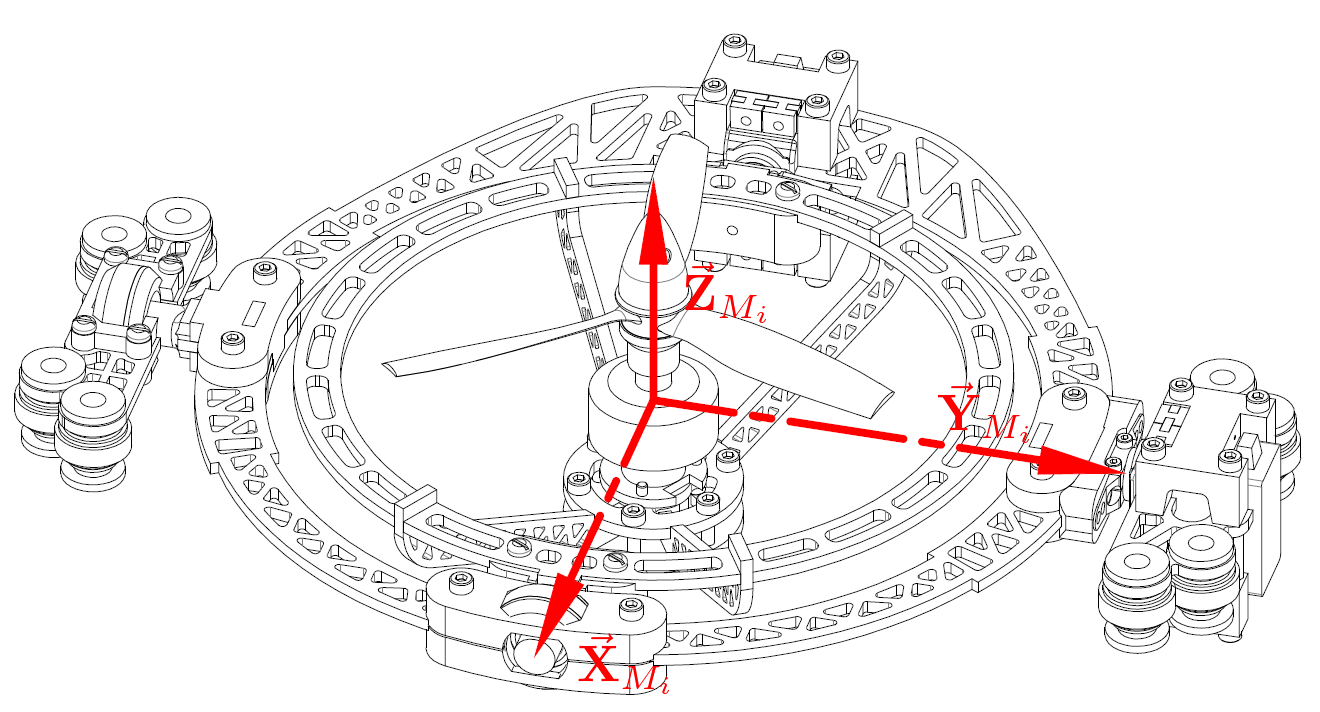
\includegraphics[width=0.85\textwidth]{figs/motor-axes}
\caption{Aligned motor frame axes}
\label{fig:motor-axes}
\vspace{-6pt}
\end{figure}
Every propeller/motor is actuated by a pair of two servos about two subsequent rotational axes (Fig:\ref{fig:motor-axes}) in a similar fashion to an Euler rotation sequence. A motor module frame $\mathcal{F}^{M_i}$ is attached to the innermost ring, the BLDC motor's stator is affixed to that frame and its rotor has a rotational velocity $\Omega_i$ about the $\hat{Z}_{M_i}$ stator axis. Fig:\ref{fig:motor-frame} shows the sequential relative module frames.
\begin{figure}[hbtp]
\vspace{-10pt}
\centering
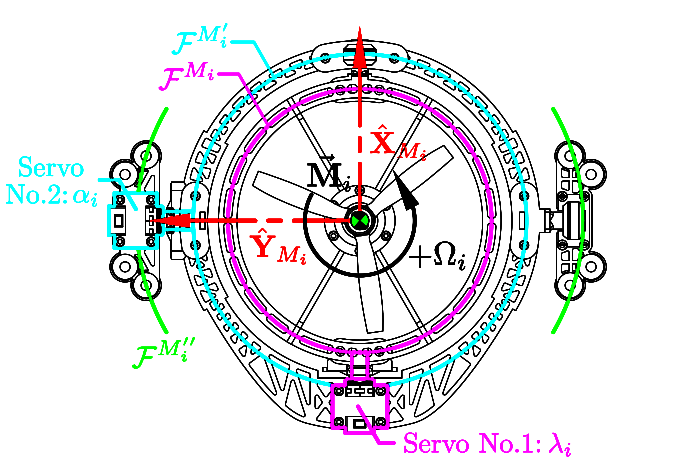
\includegraphics[width=0.9\textwidth]{figs/motor-frame}
\caption{Intermediate motor frames}
\label{fig:motor-frame}
\vspace{-8pt}
\end{figure}
\par
That inner ring frame rotates about its $\hat{X}_{M_i}$ axis by $\lambda_i$ from the module's first servo. The first servo is attached to the middle ring assembly with the frame $\mathcal{F}^{M_i'}$. The middle ring assembly and frame then rotates about its $\hat{Y}_{M_i'}$ axis actuated by the second $\alpha_i$ servo. That second servo is affixed to an intermediate $\mathcal{F}^{M_i''}$ frame, finally there's an orthogonal rotation about $\hat{Z}_{M_i''}$ between $\mathcal{F}^b$ and $\mathcal{F}^{M_i''}$. Each module's actuation state is fully described by the rotational speed, both servo positions and all their respective rates; $[\Omega_{i},~\lambda_{i},~\alpha_{i},~\dot{\Omega}_i,~\dot{\lambda}_i,~\dot{\alpha}_i]^{T}$ for $i\in [1:4]$. 
\par
Fig:\ref{fig:body-frame} shows how the axes of each motor module aligns with the body frame's axes at rest. The body frame $\mathcal{F}^b$ has the origin $\vec{\mathbf{O}}_b$ at the X-Y center of the structure, co-planar to each motor modules' center. \emph{Neither} the body frame's origin \emph{nor} each modules center of rotation are coincidental with body's center of mass. The exact disparity between the origin(s) of motion and the respective body's center of mass are quantified subsequently in Sec:\ref{sec:proto.inertia}. 
\begin{figure}[htbp]
\vspace{-6pt}
\centering
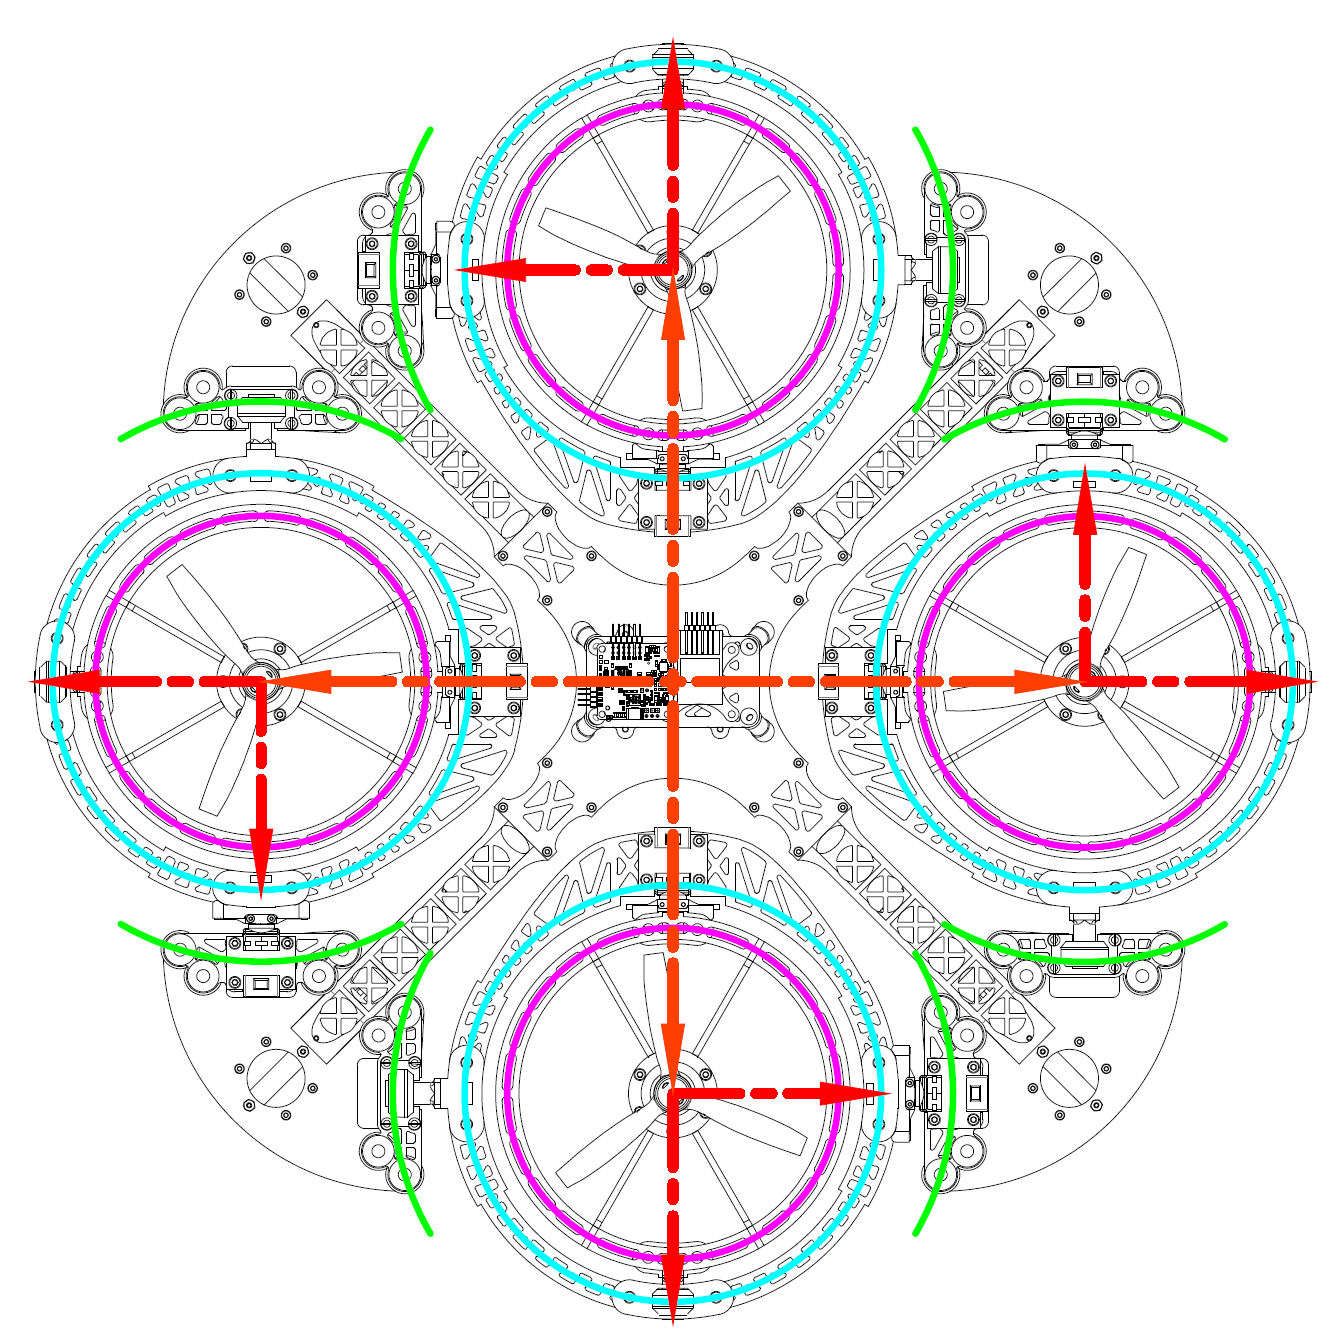
\includegraphics[width=0.85\textwidth]{figs/body-frame}
\vspace{-4pt}
\caption{Body frame axes layout}
\label{fig:body-frame}
\vspace{-16pt}
\end{figure}
\par
The motor modules pair 1 and 3 have their $\hat{X}$-axes in the positive and negative $\hat{X}_b$ directions of the body frame respectively. Similarly Modules 2 and 4 have their $\hat{X}$-axes in the positive and negative $\hat{Y}_b$ directions of the body frame. Motor modules 1 and 3 have clockwise rotating propellers; denoted by a positive superscript or $\Omega_{[1,3]}^{+}$. Conversely modules 2 and 4 have counter-clockwise rotations; denoted by a negative superscript or $\Omega_{[2,4]}^{-}$.
\par
\emph{\color{Gray}Not shown in Fig:\ref{fig:body-frame} is the relative $\hat{Z}_b$ origin position of $\vec{\mathbf{O}}_b$ with respect to the entire assembly. The $\Delta Z$ height of the body's motion centroid is such that its origin is co-planar with the four motor modules rotational centers. The center of motion is \underline{not coincidental with the center of mass}.}
\par
\begin{figure}[htbp]
\centering
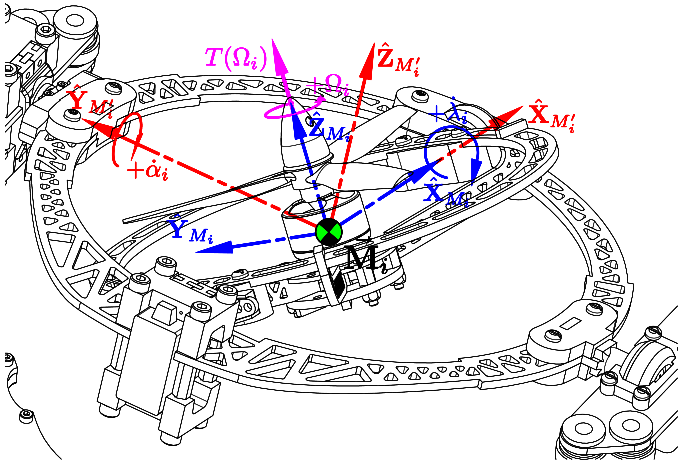
\includegraphics[width=0.75\textwidth]{figs/force-redirect}
\caption{Motor thrust force}
\label{fig:force-redirect}
\vspace{-16pt}
\end{figure}
Each motor module's rotational center $\vec{\mathbf{M}}_i$ is displaced from the body frame origin $\vec{\mathbf{O}}_b$ by the distance $L_{arm}=195.16~\text{mm}$ (shown in Fig:\ref{fig:body-frame}). Transformation of some vector $\vec{\nu}_{M_i}$ in the motor frame $\mathcal{F}^{M_i}$ to the body frame $\mathcal{F}^b$ is given as three sequential rotation operations:
\begin{subequations}
\begin{equation}\label{eq:motor-module-rotation.a}
\vec{\nu}_b=R_{M_i}^b\vec{\nu}_{M_i}=R_z(-\sigma_i)R_y(-\alpha_i)R_x(-\lambda_i)\vec{\nu}_{M_i}~~~~\in\mathcal{F}^{b},~\text{for}~~\sigma_i\in\begin{bmatrix}
0 & \frac{\pi}{2} & \pi & \frac{2\pi}{3}
\end{bmatrix}
\end{equation}
The constant orthogonal $\sigma_i$ rotations about $\hat{Z}_{M_i''}$ are independent of actuator positions, $\sigma_i$ is determined by the motor module's location, illustrated in Fig:\ref{fig:body-frame}. The rotation matrices $R_z(\sigma_i)$ for $\sigma_i=(i-1)\pi/2$ are:
\begin{equation}\label{eq:motor-module-rotation.b}
R_z=\begin{bmatrix}
1 & 0 & 0\\
0 & 1 & 0\\
0 & 0 & 1
\end{bmatrix}, \begin{bmatrix}
0 & -1 & 0\\
1 & 0 & 0\\
0 & 0 & 1
\end{bmatrix}, \begin{bmatrix}
-1 & 0 & 0\\
0 & -1 & 0\\
0 & 0 & 1
\end{bmatrix}, \begin{bmatrix}
0 & 1 & 0\\
-1 & 0 & 0\\
0 & 0 & 1
\end{bmatrix}~\text{for}~i\in[1,2,3,4]~\text{respectively}
\end{equation}
\label{eq:motor-module-rotation}
\vspace{-18pt}
\end{subequations}
\par
If the propeller's rotation produces some thrust force $T(\Omega_i)$ in the motor module frame (Fig:\ref{fig:force-redirect}) which acts through the center of rotation $\vec{\mathbf{M}}_i$; that force is similarly transformed to the body frame through Eq:\ref{eq:motor-module-rotation.a}. A thrust vector for $\vec{T}_i\in\mathcal{F}^{M_i}$ in the body frame $\mathcal{F}^b$ is calculated:
\begin{equation}\label{eq:motor-module-force-redirect}
\vec{T}_i=R_z(-\sigma_i)R_y(-\alpha_i)R_x(-\lambda_i)\begin{bmatrix}0 & 0 & T(\Omega_i)\end{bmatrix}^T~~~~\in\mathcal{F}^{b}
\end{equation}
The actuator space, including propeller speed $\Omega_i$, is then $\in\mathbb{R}^{12}$, or rather $\mathbb{U}\in\mathbb{R}^{12}$, in contrast with $\mathbb{U}\in\mathbb{R}^4$ for a standard quadrotor. The actuator input set $u \in \mathbb{U}$ is then structured as:
\begin{equation}\label{eq:actuator-space}
\underset{\in\mathbb{U}}{u}=\begin{bmatrix}
\Omega_1^+ & \lambda_1 & \alpha_1 & \ldots & \Omega_4^- & \lambda_4 & \alpha_4
\end{bmatrix}^T~~~~\in\mathbb{R}^{12}
\end{equation}
\newpage
%====================================================
\section{Inertial Matrices \& Masses}
\label{sec:proto.inertia}
%====================================================
\emph{\color{Gray}When transforming inertias between reference frames it is more appropriate to use rotation matrices to apply the transformation and not quaternions. Spatial rotation of inertial matrices are ill suited to quaternion parametrization.}
\par
An undesirable consequence of relative rotations within a non-rigid body are the inertial responses associated with such movements. Given Newton's Second Law of Rotational Motion; each applied rotation is going to produce an equal but opposite reaction onto the principally inducing body. Similarly a gyroscopic cross-product from rotational velocities is also present when rotating bodies that have their own relative rotation. Typically for most rigid body dynamics (Sec:\ref{sec:dynamics.rigidbody}), such first and second order effects are negligible given that the angular rates on which they depend are small enough to approximate as zero; $\vec{\omega}_b\approx\vec{0}$. A dynamic setpoint (non-zero) attitude tracking plant is, however, going to produce time varying body angular velocities and accelerations that must be accounted for.
\par
The dynamic effects of those torque responses are derived later in Sec:\ref{subsec:dynamics.nonlinearities.gyrotorques}. Both inertial and gyroscopic effects are dependent on the considered body's rotational inertia about each respective axis. The magnitude of those inertias are ostensibly a by-product of the structure's design but also the vehicle's instantaneous configuration.
\par
The following inertias presented are all calculated from a SolidWorks model with masses to match physical measurements of the constructed prototype. Each connected body affected by the same angular velocity is grouped together. Every motor module then contains 3 independent inertial bodies; the propeller/rotor body, the inner ring and finally middle ring assemblies, each of which are now described in detail. 
\begin{figure}[hbtp]
\vspace{-6pt}
\centering
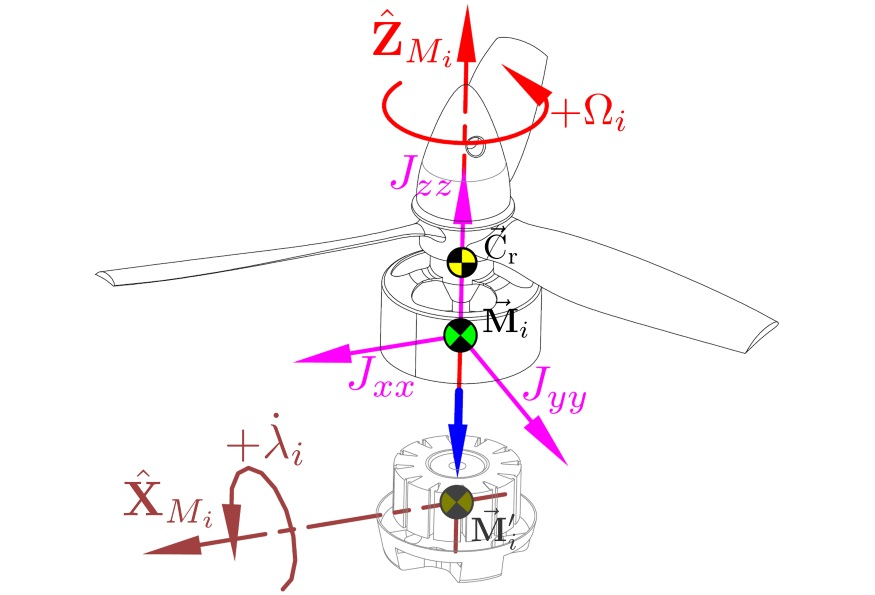
\includegraphics[width=0.71\textwidth]{figs/inertia-prop}
\caption{Rotor assembly rotational structure}
\label{fig:inertia-prop}
\vspace{-14pt}
\end{figure}
\par
The first rotational body to consider is that of the propeller and rotor assembly (Fig:\ref{fig:inertia-prop}, \underline{excluding} the motor's stator). The \emph{rotor} assembly, with subscript r, has a net mass $m_{\text{r}}=27~\text{g}$ with a center of mass $\text{C.M}_{\text{r}}=\begin{bmatrix}0.0&0.0&15.5\end{bmatrix}^T~\text{mm}$ relative to the entire motor modules center of rotation $\vec{\mathbf{M}}_i$. The propeller's rotation plane is similarly $\begin{bmatrix}0.0&0.0&23.0\end{bmatrix}^T~\text{mm}$ relative to $\vec{\mathbf{M}}_i$ (previously illustrated in Fig:\ref{fig:motor_prop}). 
\par
At high speeds the propeller's inertial contribution to the rotor assembly can be approximated as a solid disc. It follows that the inner ring's inertial components can then be regarded as constant with respect to $\Omega_i$; moreover its center of mass is independent of that propeller's rotation. 
\par
The entire rotor assembly then has a rotational constant inertia $J_\text{r}$, with principle inertial axes centered and aligned as in Fig:\ref{fig:inertia-prop}:
\begin{equation}\label{eq:prop-inertia}
J_\text{r}=\begin{bmatrix}
105.5 & 0.0 & 0.0\\
0.0 & 105.5 & 0.0\\
0.0 & 0.0 & 41.8
\end{bmatrix}~~~~\text{g.cm}^2
\end{equation}
The net angular velocity of the rotor assembly $\vec{\omega}_{r/b}$ relative to the body frame is produced by the BLDC motor's rotational velocity $\Omega_i$ and both servo rates; $\dot{\lambda}_i$ and $\dot{\alpha}_i$. Here $\Omega_i$ and both servo rates are measured in $\text{rad.s}^{\text{-}1}$, later $\Omega_i$ is used in $\text{rev.s}^{\text{-}1}$ for Blade-element momentum theory thrust calculations (Sec:\ref{subsec:dynamics.aero.bem}). Each servo's angular velocity is \emph{transformed} onto the motor frame $\mathcal{F}^{M_i}$.
\begin{equation}\label{eq:net-angular-rot}
\vec{\omega}_{r/b}=\begin{bmatrix}
0\\
0\\
\Omega_i
\end{bmatrix}
+\frac{d\lambda_i}{dt}R_x(-\lambda_i)\begin{bmatrix}
\lambda_i\\
0\\
0
\end{bmatrix}+\frac{d\alpha_i}{dt}R_y(-\alpha_i)R_x(-\lambda_i)\begin{bmatrix}
0\\
\alpha_i\\
0
\end{bmatrix}~~~~\in\mathcal{F}^{M_i}
\end{equation}
\emph{\color{gray} Eq:\ref{eq:net-angular-rot} is later replaced with a quaternion operator. That equation and the remaining angular velocity equations for each body derived here are therefore not expanded further in their current rotation matrix form(s)\ldots}
\par
\begin{figure}[htbp]
\vspace{-12pt}
\centering
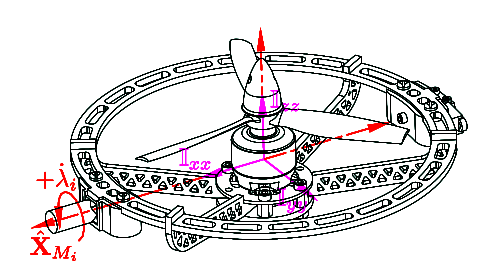
\includegraphics[width=0.75\textwidth]{figs/inertia-inner}
\vspace{-10pt}
\caption{Inner ring rotational structure}
\label{fig:inertia-inner}
\end{figure}
The next assembly, to which the motor frame $\mathcal{F}^{M_i}$ is attached, is the \emph{inner ring} assembly denoted with subscript n. The inner ring structure has a mass $m_\text{n}=92~\text{g}$, \underline{including} the rotor assembly in that calculation. The center of mass is positioned $\text{C.M}_{\text{n}}=\begin{bmatrix}-1.44&00.0&5.14\end{bmatrix}^T~\text{mm}$ relative to the module's center of rotation $\vec{\mathbf{M}}_i$. The inner ring, being rotated by the $\lambda_i$ servo about the $\hat{X}_{M_i}$ axis, then has an inertial matrix which \underline{includes} $J_\text{r}$ from Eq:\ref{eq:prop-inertia} centered and aligned with axes as in Fig:\ref{fig:inertia-inner}:
\begin{equation} \label{eq:inertia.inner}
J_\text{n}=J_{M_i}=\begin{bmatrix}
520.9 & -31.7	& -0.3\\
-31.7 & 1826.3 & 0.0\\
-0.3 & 0.0	& 2050.8\\
\end{bmatrix}~~~~\text{g.cm}^2
\end{equation}
The rotational velocity of the collective inner ring assembly $\vec{\omega}_{n/b}$ for the angular velocity of frame $\mathcal{F}^{M_i}$, is similar to that of Eq:\ref{eq:net-angular-rot}. They both occur in the same frame however the inner ring's angular velocity has no velocity contribution from $\Omega_i$:
\begin{equation}\label{eq:net-angular-inner}
\vec{\omega}_{n/b}=\frac{d\lambda_i}{dt}R_x(-\lambda_i)\begin{bmatrix}
\lambda_i\\
0\\
0
\end{bmatrix}
+\frac{d\alpha_i}{dt}R_y(-\alpha_i)R_x(-\lambda_i)\begin{bmatrix}
0\\
\alpha_i\\
0
\end{bmatrix}~~~~\in\mathcal{F}^{M_i}
\end{equation}
\par
That first actuating servo for $\lambda_i$ and its coaxial support bearing are both affixed to the intermediate \emph{middle ring} assembly, with subscript m (middle ring only Fig:\ref{fig:inertia-middle}). The intermediate frame $\mathcal{F}^{M_i'}$ is attached to the middle ring body with a mass $m_\text{m}=98~\text{g}$, \underline{excluding} the inner most ring's contribution. That middle ring body alone has a center of mass $\text{C.M}_{\text{m}}=\begin{bmatrix}
-4.70&0.37&-0.36\end{bmatrix}^T~\text{cm}$ relative to $\vec{\mathbf{M}}_i$. 
\begin{figure}[htbp]
\centering
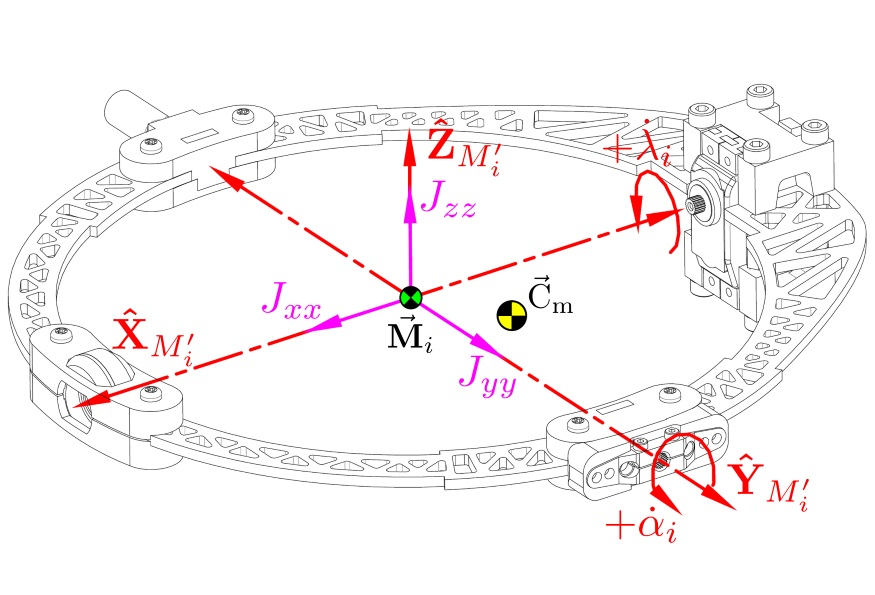
\includegraphics[width=0.7\textwidth]{figs/inertia-middle}
\vspace{-18pt}
\caption{Middle ring rotational structure}
\label{fig:inertia-middle}
\vspace{-12pt}
\end{figure}
\par
Together the inner and middle rings make the whole motor module assembly (Fig:\ref{fig:inertia-module}), with a subscript p. The net module has a mass $m_\text{p}=190~\text{g}$. The center of mass for the entire module $\text{C.M}_\text{p}$ is a function of the inner ring's rotational position $\lambda_i$ relative to the middle frame $\mathcal{F}^{M_i'}$. That module's center of mass is calculated:
\begin{subequations}\label{eq:center-module}
\begin{equation}\label{eq:center-module.a}
\text{C.M}_{\text{n}}'(\lambda)=R_x(\lambda)\big(\text{C.M}_{\text{n}}\big)
\end{equation}
\vspace{-10pt}
\begin{equation}\label{eq:center-module.b}
\text{C.M}_\text{p}(\lambda)=\frac{m_\text{m}\big(\text{C.M}_{\text{m}}\big)+m_\text{n}\big(\text{C.M}_{\text{n}}'(\lambda)\big)}{m_\text{p}}
\end{equation}
Substituting physical values into Eq:\ref{eq:center-module.b} for the inner and middle rings' center of masses respectively:
\begin{equation}\label{eq:center-module.c}
\text{C.M}_\text{p}(\lambda)=\frac{98\begin{bmatrix}-4.70 & 0.37 & -0.36\end{bmatrix}^T\times 10^{-7}+92R_x(\lambda)\begin{bmatrix}
-1.44& 0.00 & 3.06
\end{bmatrix}^T\times 10^{-8}}{190\times 10^{-3}}
\end{equation}
Which then has a value at rest, for reference, with the servo $\lambda_i=0$ relative to the center of rotation $\vec{\mathbf{M}}_i$:
\begin{equation}\label{eq:center-module.d}
\text{C.M}_\text{p}(0)=	\begin{bmatrix}
-2.49 & 0.19 & 0.04
\end{bmatrix}^T\Big|_{\lambda_i=0}~~~~\text{cm}
\end{equation}
\end{subequations}
\par
The complete motor module is finally rotated by the $\alpha_i$ servo about its $\hat{Y}_{M_i'}$ axis. The module's compound inertia $J_\text{p}$ is a combination of the middle ring's inertia $J_\text{m}$ and the inner ring's inertia $J_\text{n}$ rotated by $\lambda_i$ about $\hat{X}_{M_i}$ (Fig:\ref{fig:inertia-module}). The latter's contribution is dependent on the \emph{rotation}, not transformation, angle $\lambda_i$ which from the conservation of angular momentum theory, detailed in \cite{rigidbodyinertia}. The motor module's net rotational inertial $J_\text{p}$, is then calculated from $J_\text{m}$:
\begin{subequations}\label{eq:inertia.middle}
\begin{equation} \label{eq:inertia.middle.a}
\text{With} ~~J_\text{m}=\begin{bmatrix}
2905.7 & 0.0 & 390.9\\
0.0 & 8446.4 & 0.0\\
390.9 & 0.0 & 11125.7\\
\end{bmatrix}~~~\text{g.cm}^2
\end{equation}
\vspace{-5pt}
\begin{equation}\label{eq:inertia.middle.b}
J_\text{p}(\lambda_i)=J_\text{m}+R_{x}(\lambda_i)\big(J_\text{n}\big)R_{x}^{-1}(\lambda_i)
\end{equation}
That net inertia for the complete motor module, with $\lambda_i=0$ and relative to the middle ring frame $\mathcal{F}^{M_i'}$, has a reference value:
\begin{equation}
J_\text{p}(0)=\begin{bmatrix}
3365.4 & -0.1 & 390.6\\
-0.1 & 10210.1 & 0.0\\
390.6 & 0.0 & 13118.0             
\end{bmatrix}\Bigg|_{\lambda_i=0}~~~~\text{g.cm}^2
\end{equation}
The rotation matrix $R_x$ in Eq:\ref{eq:inertia.middle.b} is a full rank square matrix, its inverse $R^{-1}_{x}$ always exists. The module's inertia could be further divided into constant and variable components; $J_\text{p}(\lambda_i)=J_{const}+J_{M_i}(\lambda_i)$. The variable terms, if small enough or under certain conditions, could be simplified or neglected\ldots
\par
\begin{figure}[htbp]
\vspace{-10pt}
\centering
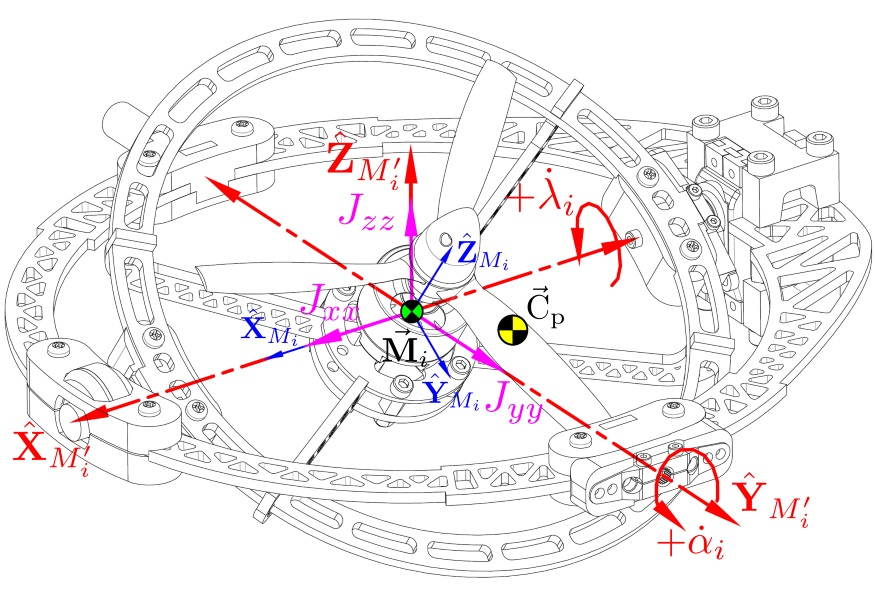
\includegraphics[width=0.7\textwidth]{figs/inertia-module}
\vspace{-12pt}
\caption{Module assembly rotational structure}
\vspace{-8pt}
\label{fig:inertia-module}
\end{figure}
Fig:\ref{fig:inertia-damping} shows how the complete motor module and its rotational axes (in Fig:\ref{fig:inertia-module}) are attached and centered relative to the body structure. The second $\alpha_i$ servo is fixed to the body structure and rotates the entire motor module about the $\hat{Y}_{M_i''}$ axis.
\begin{figure}[hbtp]
\centering
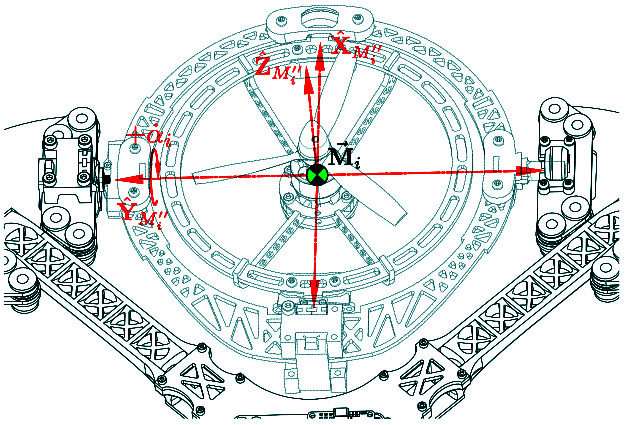
\includegraphics[width=0.85\textwidth]{figs/inertia-damping}
\vspace{-8pt}
\caption{Complete motor module attached to the body structure}
\label{fig:inertia-damping}
\vspace{-14pt}
\end{figure}
\par
Finally, the angular velocity experienced by the net motor assembly relative to the body frame, $\vec{\omega}_{p/b}$ in frame $\mathcal{F}^{M_i'}$, is entirely as a result of the $\alpha_i$ servo actuation:
\begin{equation}
\vec{\omega}_{p/b}=\frac{d\alpha_i}{dt}R_y(-\alpha_i)\begin{bmatrix}
0\\
\alpha_i\\
0
\end{bmatrix}~~~~\in\mathcal{F}^{M_i'}
\end{equation}
\end{subequations}
That $\alpha_i$ servo is affixed to the body structure and so its inertial volume and that of the outer coaxial bearing support contributes then to the body structure's inertia; whose value excludes any of the four motor modules. Attached to that servo is an intermediate frame $\mathcal{F}^{M_i''}$ (Fig:\ref{fig:inertia-damping}) which differs from the middle ring frame by an $R_y(-\alpha_i)$ transformation and differs from the body frame $F^b$ by an orthogonal $R_z(\sigma_i)$ rotation.
\par
The motor modules are suspended from the body frame with a set of silicone damping balls. The \emph{body structure} which includes those connecting masses, with a subscript y, has center of mass $\text{C.M}_{\text{y}}$ (without any motor modules attached, Fig:\ref{fig:inertia-center}). The center of mass coincides with the $\hat{X}_b$ and $\hat{Y}_b$ directional axes but lies $\Delta Z=-9.52~\text{mm}$ below the body frame's origin of motion $\vec{\mathbf{O}}_b\in\mathcal{F}^b$.
\par
\begin{figure}[hbtp]
\vspace{-8pt}
\centering
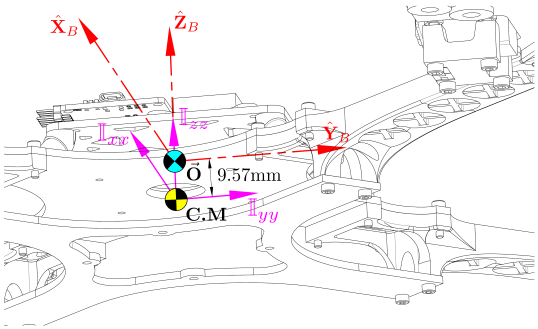
\includegraphics[width=0.81\textwidth]{figs/inertia-center}
\caption{Body structure's center of mass}
\label{fig:inertia-center}
\vspace{-6pt}
\end{figure}
\par
\emph{\color{Gray}Note: that body frame origin $\vec{\mathbf{O}}_b$ which all motion is calculated with respect to is co-planar to the motor module's rotational centers, \underline{not the net center of mass}.}
\par
The body structure's weight, including all four damping assemblies and electronics, totals to $m_\text{y}=814.70~\text{g}$. Similarly the body structure's net inertia (\emph{sans} motor modules) $J_\text{y}$, about its center of mass (Fig:\ref{fig:inertia-center}), is:
\begin{subequations}\label{eq:inertia.body}
\begin{equation}\label{eq:inertia.body.a}
\underset{C.M}{J_\text{y}}=\begin{bmatrix}
181569.7 & 0.4 &-19.4\\
0.4 & 181692.2 & 8.9\\
-19.4 & 8.8 & 360067.2\\
\end{bmatrix}\times 10^{-7}~~~\text{kg.m}^2
\end{equation}
Using the Parallel Axis theorem to translate that inertia to the origin of motion by $\Delta Z=+9.52~[\text{mm}]$, the inertia about the origin, $\vec{\mathbf{O}}_b$, is:
\begin{equation}\label{eq:inertia.body.b}
J'=J+m\big(\vec{d}\cdot\vec{d}-\vec{d}\otimes\vec{d}\hspace{3pt}\big)\approx J+md^2
\end{equation}
\emph{\color{Gray}For the general parallel axis transformation in Eq:\ref{eq:inertia.body.b}, $\otimes$ represents the Hamilton product of two $[3\times 1]$ matrices. It is used later to indicate quaternion multiplication. The vector $\vec{d}$ is the difference between the center of mass $\mathbf{C.M}_\text{y}$ and the body frame origin $\vec{\mathbf{O}}_b$.}
\begin{equation}
\therefore J_y'=\underset{C.M}{J_\text{y}}+m_\text{y}\big(\Delta\vec{Z}\cdot\Delta\vec{Z}-\Delta\vec{Z}\otimes\Delta\vec{Z}\big)
\end{equation}
That body's constant inertia $J_\text{y}$ at the origin $\vec{\mathbf{O}}_b$ and aligned with the body frame $\mathcal{F}^{b}$ is then:
\begin{equation}\label{eq:inertia.body.c}
\rightarrow\underset{\vec{\mathbf{O}}_b}{J_\text{y}'}=\begin{bmatrix}
182307.7 & 0.4 & -14.5\\
0.4 & 182430.1 & 6.5\\
-14.5& 6.5 & 360067.2
\end{bmatrix} \times10^{-7}~~~\text{kg.m}^2
\end{equation}
\end{subequations}
Net inertia for the complete multibody vehicle, $J_b(u)$ about the origin $\vec{\mathbf{O}}_b$, is a combination of all the relative attached bodies as a function of all actuator positions $u\in\mathbb{U}$. The entire assembly's inertia $J_b(u)$ is the \emph{net} body frame's inertia, different from $J_\text{y}$ which is the inertia for \emph{only} the body structure. That collective assembly being the four motor modules, each rotated first by $\lambda_i$, then $\alpha_i$ and finally translated to the body frame origin; and the body structure's contribution itself. 
\par
Those motor modules' inertial transformations from their respective centers of rotation, in frames $\mathcal{F}^{M_i}$ for $i\in[1:4]$, to the body frame $\mathcal{F}^b$ are analogous to that of Eq:\ref{eq:motor-module-rotation}. Reiterating that $\vec{\mathbf{O}}_b$ is \emph{co-planar} to each module's center of rotation; each motor module's inertia $J_\text{p}(\lambda_i)$, defined in Eq:\ref{eq:inertia.middle.b}, is further rotated by $\alpha_{i}$ about the $\hat{Y}_{M_i'}$ axis and finally an orthogonal $\hat{Z}_{M_i''}$  axis rotation (aligned with $\hat{Z}_b$) onto $\mathcal{F}^b$. 
\par
\begin{figure}[hbtp]
\vspace{-6pt}
\centering
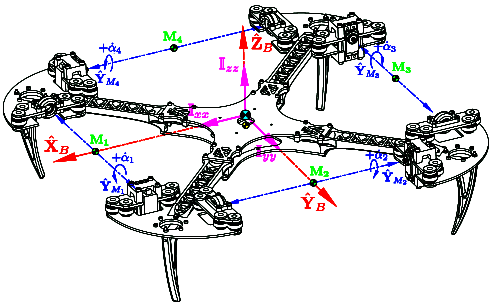
\includegraphics[width=\textwidth]{figs/inertia-frame}
\caption{Inertial, mass and motor modules respective centers}
\label{fig:inertia-frame}
\vspace{-6pt}
\end{figure}
For the entire body's net inertia each contributing assembly's inertia must be defined with respect to the body's origin; first aligned parallel to the common set of body frame axes $\hat{X}_b,\hat{Y}_b$ and $\hat{Z}_b$ and then translated to the origin $\vec{\mathbf{O}}_b$. Each motor module's inertia, still centered relative to each individual rotational center $\vec{\mathbf{M}}_i$ in Fig:\ref{fig:inertia-frame}, but re-orientated to align parallel TO $\vec{\mathbf{O}}_b$ with rotations about axes $\hat{X}\in\mathcal{F}^{M_i},~\hat{Y}\in\mathcal{F}^{M_i'},~\hat{Z}\in\mathcal{F}^{M_i''}$, is calculated:
\begin{subequations}\label{eq:module-inertia}
\begin{equation}\label{eq:module-inertia.a}
J_{\vec{\mathbf{M}}_i}(u\cdot i)=R_{z}(\sigma_i)R_{y}(\alpha_i)\big(J_{p}(\lambda_i)\big)R^{-1}_{y}(\alpha_i)R^{-1}_{z}(\sigma_i)~\text{for}~i\in[1:4]
\end{equation}
The argument $(u\cdot i)$ in Eq:\ref{eq:module-inertia.a} is the i\textsuperscript{th} projection of the actuator space; that being $\begin{bmatrix}\Omega_i&\lambda_i&\alpha_i\end{bmatrix}^T$.
Furthermore the rotation $R_{z}(\sigma_i)$ was defined as an orthogonal $\hat{Z}_b$ rotation previously in Eq:\ref{eq:motor-module-rotation.b}. Expanding each module's inertia to individual inner and middle ring inertial contributions then yields:
\begin{equation}\label{eq:module-inertia.c}
\therefore J_{\vec{\mathbf{M}}_i}(u\cdot i)=R_{z}R_{y}(\alpha_i)\big(J_\text{m}\big)R^{-1}_{y}(\alpha_i)R^{-1}_z+R_{z}R_{y}(\alpha_i)R_{x}(\lambda_i)\big(J_\text{n}\big)R^{-1}_{x}(\lambda_i)R^{-1}_{y}(\alpha_i)R^{-1}_z
\end{equation}
\end{subequations}
\emph{\color{Gray}It's at this stage that, despite simplifications, the symbolic inertial equations all become overly cumbersome to include with numeric values\ldots~For the sake of brevity, exact calculated inertial values for the input dependent plant are omitted.}
\par
Each module's rotational center, vectors $\vec{\mathbf{M}}_{1\rightarrow 4}$, are all equally spaced relative to the origin of motion, $\vec{\mathbf{O}}_b$, with a parallel axis arm $L_{arm}=195.16~~\text{mm}$ (Fig:\ref{fig:inertia-frame}). To avoid notational confusion the term $\vec{L}_i=\begin{bmatrix} \pm 195.16 & 0 & 0 \end{bmatrix}^T$ or $\begin{bmatrix} 0 & \pm 195.16 & 0
\end{bmatrix}^T$ is used to represent the vector displacement between the origin $\vec{\mathbf{O}}_b$ and each motor modules center of rotation $\vec{\mathbf{M}}_{1\rightarrow 4}$. The net inertial equation $J_b(u)$, about the origin $\vec{\mathbf{O}}_b$ and depending on the actuator position matrix $u\in\mathbb{U}$, can be calculated as:
\begin{subequations}
\label{eq:body-inertia}
\begin{equation}\label{eq:body-inertia.a}
\underset{\vec{\mathbf{O}}_b}{J_b}(u)=J_\text{y}+\sum_{i=1}^{4}J'_{\vec{\mathbf{M}}_i}(u\cdot i)~~~~\text{kg.m}^2,~u\in\mathbb{U}
\end{equation}
Where $J'_{\vec{\mathbf{M}}_i}(u\cdot i)$ is the motor module inertia from Eq:\ref{eq:module-inertia} but translated to the origin $\vec{\mathbf{O}}_b$ using a parallel axis theorem with $m_\text{p}=190~\text{g}$ and the displacement vector $\vec{L}_i$:
\begin{equation}\label{eq:body-inertia.b}
J'_{\vec{\mathbf{M}}_i}(u\cdot i)=J_{\vec{\mathbf{M}}_i}(u\cdot i)+m_\text{p}\big(\vec{L}_i \cdot \vec{L}_i - \vec{L}_i\otimes\vec{L}_i\big)
\end{equation}
\end{subequations}
Although Eq:\ref{eq:body-inertia} produces the net multi-body's inertia, each equation to calculate $J_{\vec{\mathbf{M}}_i}'$ involves cascaded transformations which may deteriorate the result's certainty. Each module's inertia is first translated to their respective centers of rotation then rotated as per the two servos and then finally translated again back to the body frame's origin. 
\par
Alternatively the inertia contribution of each sub-assembly can be considered separately and translated directly to the body frame's origin from their respective mass centers. This will improve the accuracy of the produced inertial equations, each translation/rotation has with it an associated floating point concatenation. It is also perhaps more intuitive for the reader to consider each sub-body's contribution individually, despite having been derived as combined inertial bodies in the above. The vehicles net inertia can then be described as nine separate contributing bodies; four inner rings $J_\text{n}$, four middle rings $J_\text{m}$ and one body structure $J_\text{y}$:
\begin{equation}\label{eq:body-net}
\underset{\vec{\mathbf{O}}_b}{J_b}(u)=\underset{\vec{\mathbf{O}}_b}{J'_\text{y}}+\sum_{i=1}^{4} \underset{\vec{\mathbf{O}}_b}{J_\text{n}}(u\cdot i)+\sum_{i=1}^{4} \underset{\vec{\mathbf{O}}_b}{J_\text{m}}(u\cdot i)~~~~u\in\mathbb{U}
\end{equation}
Note that the rotor's inertia $J_r$ is included in $J_n$. Then isolating each body and considering each inertia independently. Starting with the inner ring's contribution; having an inertia $J_\text{n}$ with respect to its \emph{center of mass}, and not center of rotation, measured \emph{relative} to its center of rotation. The following is then fundamentally different from the process in Eq:\ref{eq:inertia.inner}, calculating the inner ring's inertial contribution about the origin $\vec{\mathbf{O}}_b$.
\par
\begin{subequations}
\label{eq:body-net-inner}
For the inner ring only, with a mass $m_\text{n}$ and center of mass $C.M_\text{n}$ relative to its center of rotation $\vec{\mathbf{M}}_i$. The inner ring's directly transformed inertial contribution then follows:
\begin{equation}\label{eq:body-net-inner.a}
m_\text{n}=92~~~~\text{g}
\end{equation}
\vspace{-10pt}
\begin{equation}\label{eq:body-net-inner.b}
C.M_\text{n}=\begin{bmatrix}
-1.44 & 0.0 & 5.14
\end{bmatrix}^T~~~~\text{mm},~\in\mathcal{F}^{M_i}
\end{equation}
The inner ring's inertial matrix about it's center of mass (Fig:\ref{fig:inertia-inner}) is the constant:
\begin{equation}\label{eq:body-net-inner.c}
\underset{C.M}{J_\text{n}}=\begin{bmatrix}
496.6 & -31.7 & 6.6\\
-31.7 & 1800.1 & 0.0\\
6.6 & 0 & 2048.9
\end{bmatrix}~~~~\text{g.cm}^2
\end{equation}
Relative to the body frame's origin $\vec{\mathbf{O}}_b$ the inner ring has a center of mass, rotated by $\lambda_i$ and $\alpha_i$ servos about their respective axes with a relative orthogonal $R_z$ rotation with $\sigma_i$ for the $i^\text{th}$ module implied:
\begin{equation}\label{eq:body-net-inner.d}
C.M'''_\text{n}(\lambda_i,\alpha_i)=R_zR_y(\alpha_i)R_x(\lambda_i) \big(C.M_\text{n}\big)~~~~\in\mathcal{F}^{b}
\end{equation}
Transforming the inertia from Eq:\ref{eq:body-net-inner.c}, still about the center of mass $C.M_\text{n}'''$, but with axes aligned parallel with to body frame, or using the shorthand $||\vec{\mathbf{O}}_b$. The inner ring's inertia as a function of both servo angles $\lambda_i$ and $\alpha_i$ aligned with $\mathcal{F}^b$ is:
\begin{equation}\label{eq:body-net-inner.e}
\underset{||\vec{\mathbf{O}}_b}{J'''_\text{n}}(\lambda_i,\alpha_i)=R_zR_y(\alpha_i)R_x(\lambda_i)\big(J_\text{n}\big)R^{-1}_x(\lambda_i)R^{-1}_y(\alpha_i)R^{-1}_z
\end{equation}
The vector difference between the rotated center of mass $C.M_\text{n}'''$ with the body origin $\vec{\mathbf{O}}_b$ is:
\begin{equation}
\Delta L = \vec{L}_i-C.M'''_\text{n}(\lambda_i,\alpha_i)
\end{equation}
Then using the above with a parallel axis translation, adapted from Eq:\ref{eq:inertia.body.b}, to move the rotated inertia $J'''_\text{n}$ to the center of the body frame $\vec{\mathbf{O}}_b$:
\begin{equation}
\underset{\vec{\mathbf{O}}_b}{J_\text{n}}(\lambda_i,\alpha_i)=\underset{||\vec{\mathbf{O}}_b}{J'''_\text{n}}(\lambda_i,\alpha_i)+ m_\text{n} \big((\Delta L \cdot \Delta L)\mathbb{I}_{3\times 3} - \Delta L \otimes \Delta L \big)
\end{equation}
And for reference when both servos are at rest; $\lambda_i=0$ and $\alpha_i=0$, the inner ring's inertial contribution about the origin is explicitly:
\begin{equation}
\underset{\vec{\mathbf{O}}_b}{J_\text{n}}(\lambda_i,\alpha_i)=\begin{bmatrix}
520.9 & -31.0 & 922.6\\
-31.0 & 36348.5 & 0.0\\
922.6 & 0.0 & 36573.0
\end{bmatrix}\times 10^{-7}\bigg|_{\lambda_i,\alpha_i=0}~~~~\text{kg.m}^2,~\in\mathcal{F}^{b}
\end{equation}
\end{subequations}
Similarly, the same process is applied for the middle ring's rotated and translated inertia. The middle ring \emph{only} (Fig:\ref{fig:inertia-middle}) has a mass and center of mass relative to the module's center of rotation respectively:
\begin{subequations}
\label{eq:body-net-middle}
\begin{equation}\label{eq:body-net-middle.a}
m_\text{m}=98~~~~\text{g}
\end{equation}
\vspace{-14pt}
\begin{equation}
C.M_\text{m}=\begin{bmatrix}
-47.00 & 3.74 & -3.63
\end{bmatrix}^T~~~~\text{mm},~\in\mathcal{F}^{M_i'}
\end{equation}
The inertial matrix of the middle ring body, excluding the inner ring, about its center of mass is:
\begin{equation}
\underset{C.M}{J_\text{m}}=\begin{bmatrix}
2879.1 & 172.3 & 223.6\\
172.3 & 6269.0 & 13.3\\
223.6 & 13.3 & 8947.5\\
\end{bmatrix}~~~~\text{g.cm}^2
\end{equation}
Rotating the center of mass only by the $\alpha_i$ servo about the $\hat{Y}_{M_i'}$ axis yields the center of mass $C.M_\text{m}'$ relative to $\vec{\mathbf{O}}_b$:
\begin{equation}\label{eq:body-net-middle.d}
C.M''_\text{m}(\alpha_i)=R_{z}R_{y}(\alpha_i)\big(C.M_\text{m}\big)~~~~\in\mathcal{F}^{b}
\end{equation}
Then the rotated inertial matrix, aligned with axes parallel to the body frame origin $\vec{\mathbf{O}}_b$, follows:
\begin{equation}
\underset{||\vec{\mathbf{O}}_b}{J''_\text{m}}(\alpha_i)=R_zR_y(\alpha_i)\big(J_\text{m}\big)R^{-1}_y(\alpha_i)R^{-1}_z
\end{equation}
The vector difference from the rotated center of mass to the body frame origin is calculated:
\begin{equation}
\Delta L = \vec{L}_i-{C.M''_\text{m}}(\alpha_i)
\end{equation}
Which then leads to the parallel axis translation of the middle ring's inertia to the body origin:
\begin{equation}
\underset{\vec{\mathbf{O}}_b}{J_\text{m}}(\alpha_i)=\underset{||\vec{\mathbf{O}}_b}{J''_\text{m}}(\alpha_i)+m_\text{m}\big((\Delta L\cdot\Delta L)\mathbb{I}_{3x3}-\Delta L \otimes \Delta L \big)
\end{equation}
Again for reference; at rest with the middle ring servo $\alpha_i=0$ the middle ring's inertial contribution at $\vec{\mathbf{O}}_b$ is:
\begin{equation}
\underset{\vec{\mathbf{O}}_b}{J_\text{m}}(\alpha_i)=\begin{bmatrix}
2905.7 & 715.4 & -303.9\\
715.4 & 27795.7 & 0.0\\
-303.9 & 0.0 & 30475.0
\end{bmatrix}
\times 10^{-7}\Big|_{\alpha_i=0}~~~~\text{kg.m}^2,~\in\mathcal{F}^{b}
\end{equation}
\end{subequations}
Then, reiterating Eq:\ref{eq:body-net}, the instantaneous inertia of the entire body in motion is calculated as the contribution of each connected sub-body, depending on the actuator matrix $u\in\mathbb{U}$.
\begin{subequations}
\begin{equation}\label{eq:body-net-2}
\underset{\vec{\mathbf{O}}_b}{J_b}(u)=\underset{\vec{\mathbf{O}}_b}{J'_\text{y}}+\sum_{i=1}^{4} \underset{\vec{\mathbf{O}}_b}{J_\text{n}}(u\cdot i)+\sum_{i=1}^{4} \underset{\vec{\mathbf{O}}_b}{J_\text{m}}(u\cdot i)~~~~u\in\mathbb{U}
\end{equation}
The net mass for the entire multibody system is $m_b=1574.7~\text{g}$. For reference and using Eq:\ref{eq:body-net-2}; the inertial matrix for the assembly when actuators are at rest conditions, $u=\vec{0}$, about the origin $\vec{\mathbf{O}}_b$ is:
\begin{equation}
J_b(\vec{0})=\begin{bmatrix}
317448.2 & 0.4 & -14.5\\
0.4 & 317570.7 & 6.5\\
-14.5 & 6.5 & 628257.5
\end{bmatrix}\times 10^{-7}\bigg|_{u=\vec{0}}~~~~\text{kg.m}^2,~\in\mathcal{F}^b
\end{equation}
\end{subequations}
The maximum variation of the body's net inertia is found from the maximum determinant of the inertial matrix in Eq:\ref{eq:body-net-2} for some actuator state $max(det|J_b(u_\Lambda)|)~,u_\Lambda\in\mathbb{U}$. A maximum $J_b(u_\Lambda)$, with a determinant $det|J_b(u_\Lambda)|=1017.93\times 10^{-7}$, is:
\begin{subequations}\label{eq:inertia-max}
\begin{equation}
J_b(u_\Lambda)=\begin{bmatrix}
384695.4 & 0.4 & -14.5\\
0.4 & 384717.9 & 6.5\\
-14.5 & 6.5 & 687970.7
\end{bmatrix}\times 10^{-7}\bigg|_{u_\Lambda}~~~~\text{kg.m}^2,~\in\mathcal{F}^b
\end{equation}
With an actuator matrix, independent of propeller speeds $\Omega_{1\rightarrow 4}$, as follows:
\begin{equation}
u_\Lambda=\begin{bmatrix*}[l]
\Omega_1, & \lambda_1=178\text{\textdegree},&\alpha_1=260\text{\textdegree}\ldots\\
\Omega_2, & \lambda_2=178\text{\textdegree},&\alpha_2=260\text{\textdegree}\ldots\\
\Omega_3, & \lambda_3=178\text{\textdegree},&\alpha_3=~~~0\text{\textdegree}\ldots\\
\Omega_4, & \lambda_4=~~~0\text{\textdegree}, & \alpha_4=~~~0\text{\textdegree}
\end{bmatrix*}
\end{equation}
\end{subequations}
Conversely, the minimum net inertia for the body is from the smallest determinant of Eq:\ref{eq:body-net-2}, for the actuator state $min(det|J_b(u_\Upsilon)|),~u_\Upsilon\in\mathbb{U}$. A minimum $J_b(u_\Upsilon)$, with a determinant $det|J_b(u_\Upsilon)|=633.48\times 10^{-7}$, is:
\begin{subequations}\label{eq:inertia-min}
\begin{equation}
J_b(u_\Upsilon)=\begin{bmatrix}
317469.0 & 0.4 & -1219.0\\
0.4 & 317591.5 & 1195.3\\
-1219.0 & 1195.3 & 628298.1
\end{bmatrix}\times 10^{-7}\bigg|_{u_\Upsilon}~~~~\text{kg.m}^2,~\in\mathcal{F}^b
\end{equation}
When an actuator matrix for that minimum inertia is:
\begin{equation}
u_\Upsilon=\begin{bmatrix*}[l]
\Omega_1, & \lambda_1=178\text{\textdegree},&\alpha_1=~~~0\text{\textdegree}\ldots\\
\Omega_2, & \lambda_2=~~~0\text{\textdegree},&\alpha_2=260\text{\textdegree}\ldots\\
\Omega_3, & \lambda_3=~~~0\text{\textdegree},&\alpha_3=~~~0\text{\textdegree}\ldots\\
\Omega_4, & \lambda_4=~~~0\text{\textdegree}, & \alpha_4=~~~0\text{\textdegree}
\end{bmatrix*}
\end{equation}
\end{subequations}
The inclusion of Eq:\ref{eq:inertia-max} and Eq:\ref{eq:inertia-min} are used for maximum and minimum Eigenvalues of the body's inertial matrix at a later stage in the control derivation, Sec:\ref{sec:control.attitude}. It is interesting to note that both extremes of $J_b(u)$ are still symmetrical, and \emph{roughly} diagonal. Actuator positions hardly affect the skew products of inertia in $J_b(u)$ but can vary the diagonal moments of inertia by almost $20\%$ of their principle value.
\par
Unless otherwise specified; any inertia $J_b(u)$ indicates an instantaneous calculated solution to Eq:\ref{eq:body-net-2} given a particular $u(t)\in\mathbb{U}$. The purpose of the derivations for rotated centers of mass in Eq:\ref{eq:body-net-inner} and Eq:\ref{eq:body-net-middle} is twofold; highlighting both the inertial contributions \emph{and} the variable center of mass for each sub-body. Seeing that the origin of motion $\vec{\mathbf{O}}_b$ in the body frame $\mathcal{F}^b$ and the body's effective center of mass $C.M_\text{b}$ are not coincidental, it is important to quantify the net center of mass's variation with actuator positions $u\in\mathbb{U}$. 
\par
In the general case for a collection of $n$ bodies, with each body's center of mass at some position $\vec{X}_i$ and each having a mass $m_i$, resultant center of mass is:
\begin{subequations}\label{eq:mass-center}
\begin{equation}\label{eq:mass-center.a}
C.M = \frac{\sum_{i=1}^{n} m_i.\vec{X}_i}{\sum_{i=1}^{n} m_i}
\end{equation}
Using $C.M_\text{n}'''(\lambda_i,\alpha_i)$ and $C.M_\text{m}''(\alpha_i)$ as rotated centers of mass defined in Eq:\ref{eq:body-net-inner.d} and Eq:\ref{eq:body-net-middle.d} respectively and $C.M_\text{y}$ for the body structure, the vehicle has a variable center of mass $C.M_\text{b}(u)$:
\begin{equation}\label{eq:mass-center.b}
C.M_\text{b}(u)=\frac{m_\text{y}C.M_\text{y}+\sum_{i=1}^{4} m_\text{n}C.M_\text{n}'''(u\cdot i)+\sum_{i=1}^{4} m_\text{m}C.M_\text{m}''(u\cdot i)}{m_\text{b}}
\end{equation}
\end{subequations}
So, for reference, the net center of gravity for the entire multibody assembly, when all actuators are at their zero positions is: $C.M_b(\vec{0})=\begin{bmatrix}0 & 0 & -4.94\end{bmatrix}^T~\text{mm}$. Using a gravity force vector $\vec{G}_b$ in the body frame as a result of gravitational acceleration $g=-9.81~\text{m.s}^{\text{-}2}$, acting on the vehicle's center of mass:
\begin{subequations}\label{eq:grav-def}
\begin{equation}
\vec{G}_b=R_I\big(\vec{\eta}\hspace{2pt}\big)^b\vec{G}_I~~~~\in\mathcal{F}^b
\end{equation}
\vspace{-14pt}
\begin{equation}
=R_I^b\big(\vec{\eta}\big)\begin{bmatrix}0&0&-9.81(m_\text{b})\end{bmatrix}^T~~~~\text{N}
\end{equation}
Because Eq:\ref{eq:grav-def} acts through the body's center of gravity $C.M_\text{b}(u)$, not its center of motion $\vec{\mathbf{O}}_b$, there exists a gravitational torque from the varying center of gravity. The resultant gravitational torque about the origin $\vec{\mathbf{O}}_b$ in the body frame $\mathcal{F}^b$ from that eccentric mass center for the vehicle is:
\begin{equation}
\Delta C.G = \vec{\mathbf{O}}_b-C.M_\text{b}(u)
\end{equation}
\vspace{-15pt}
\begin{equation}\label{eq:grav-torque}
\vec{\tau}_g=\Delta C.G\times m_b\vec{G}_b~~~~\in\mathcal{F}^b
\end{equation}
\end{subequations}
The prototype which was constructed is shown in Fig:\ref{fig:ducky}. The above mass centers and inertias were calculated from physical values measured on assembled components of the prototype. The listed values includes measurements of fasteners and electronics.
\begin{figure}[hbtp]
\centering
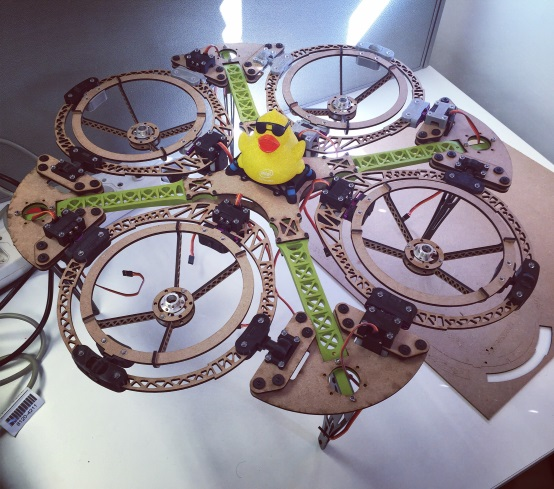
\includegraphics[width=0.7\textwidth]{figs/ducky}
\vspace{-6pt}
\caption{Final constructed prototype}
\vspace{-12pt}
\label{fig:ducky}
\end{figure}
\par
Uncertainty with inertial measurements, proven to be destabilizing and detrimental to control efforts in \cite{inertiafree,inertiaspin}, can indeed be incorporated into state dependent plant uncertainty  compenstaion like in \cite{intelligentbackstep}. Controllers with strong disturbance and uncertainty rejection, like a well designed $\text{H}_\infty$ controller, would be ideally suited to controlling an attitude plant without having to explicitly specify all of the above inertias. 
\par
It is, however, worth the mathematical deliberation to detail each inertial equation given that Lagrange dynamics are later applied to determine the servo actuator dynamic responses (Sec:\ref{sec:dynamics.nonlinearities}). Such equations of motion will later need explicit terms defined for instantaneous transformed inertias\ldots
\newpage
%====================================================
\section{Electronics}
\label{sec:proto.layout}
%====================================================
{\centering
\vspace{-20pt}
\begin{minipage}{\textwidth}
\centering
\fbox{
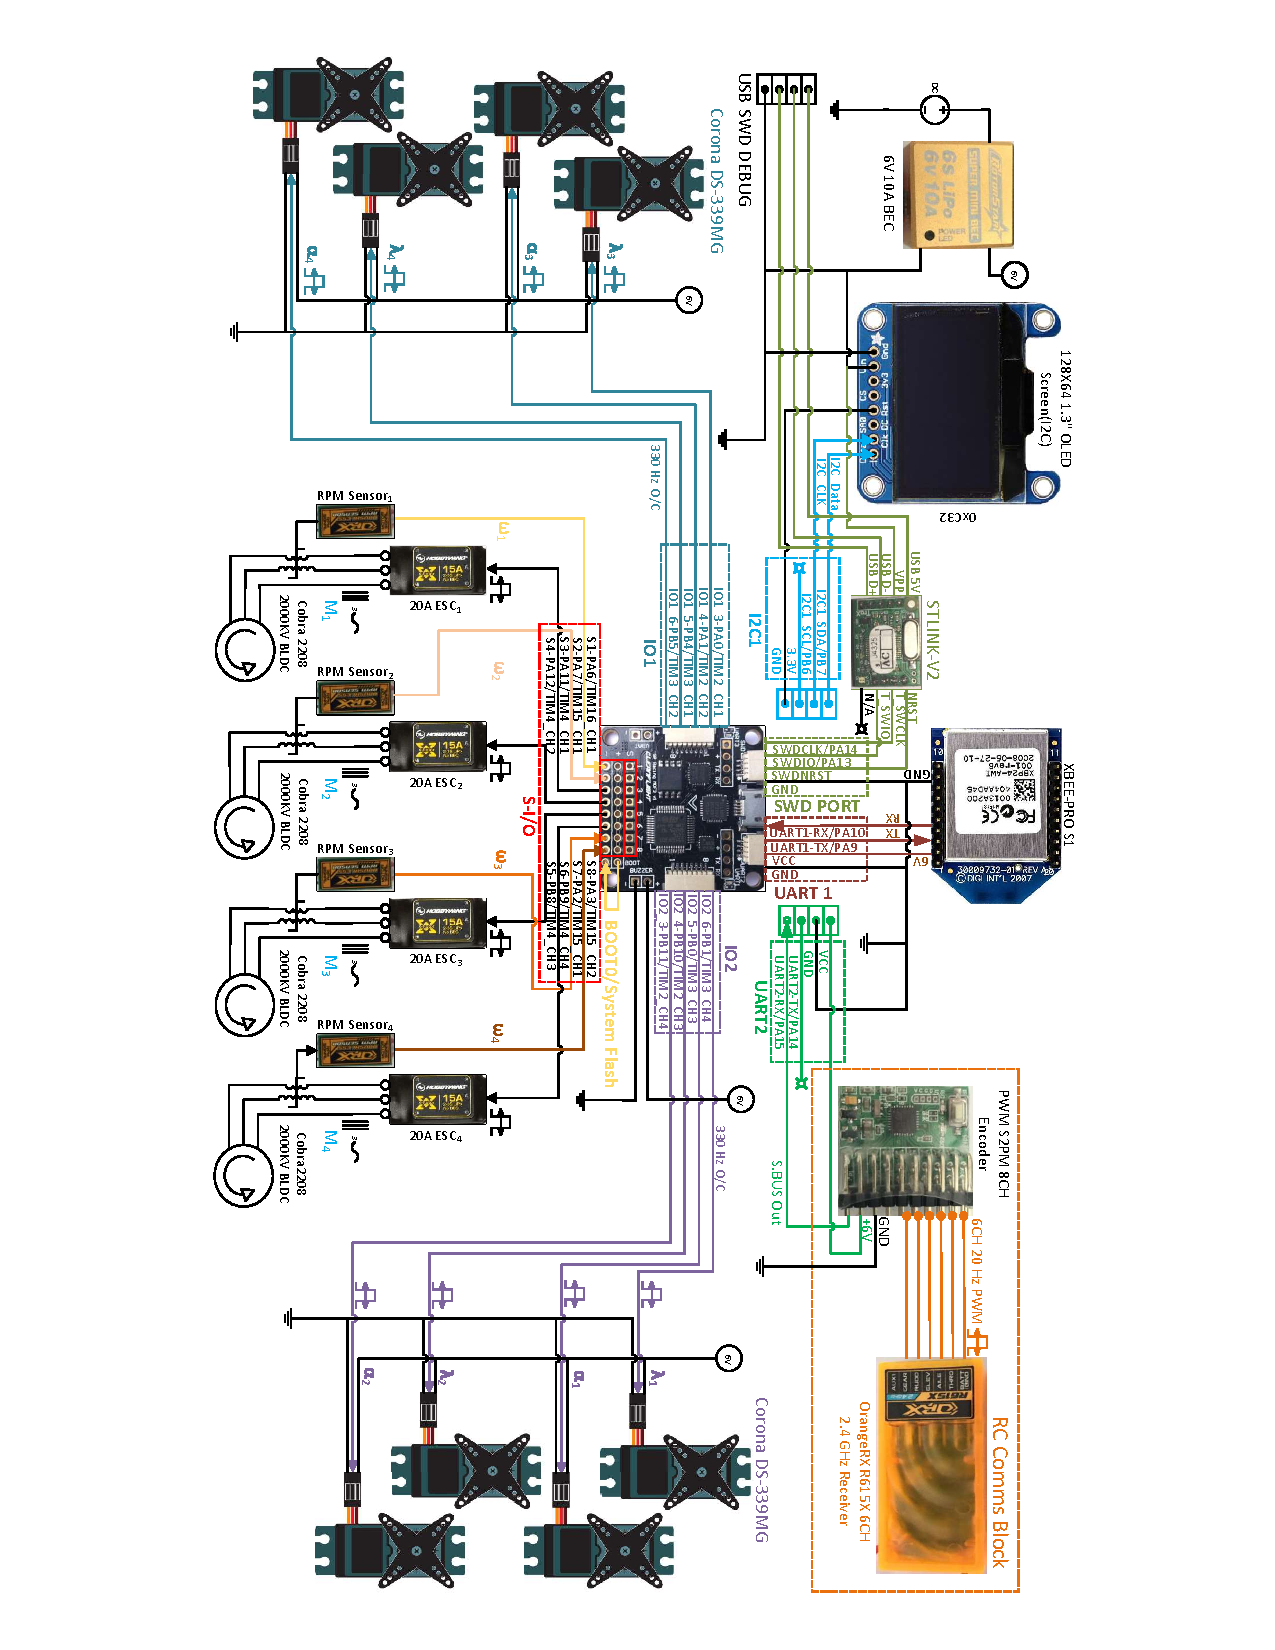
\includegraphics[clip, trim=3.5cm 1cm 3.4cm 1cm, width=0.81\textwidth]{pdfpages/electrical-schematic.pdf}
}
\end{minipage}
\vspace{-10pt}
\captionof{figure}{Hardware schematic diagram}
\label{fig:electrical-schematic}
}
%-----------------------------------------------------
\newpage
%-----------------------------------------------------
An abstracted hardware diagram for the proposed (electronic) system layout is shown in Fig:\ref{fig:electrical-schematic}. It is an illustration for the connection of different electronic peripherals to aid the on-board control system. The structure of the implemented autopilot system and control loops are addressed later. This section aims to provide a brief overview of the specific modules intended for the flight controller, their purpose and a description of how they are interfaced. No control loops or code structures are discussed here.
\par
\begin{figure}[htbp]
\begin{subfigure}{0.5\textwidth}
\centering
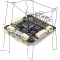
\includegraphics[width=0.95\textwidth]{figs/f3-deluxe}
\caption{SPRacing F3 deluxe flight controller}
\end{subfigure}
\begin{subfigure}{0.5\textwidth}
\centering
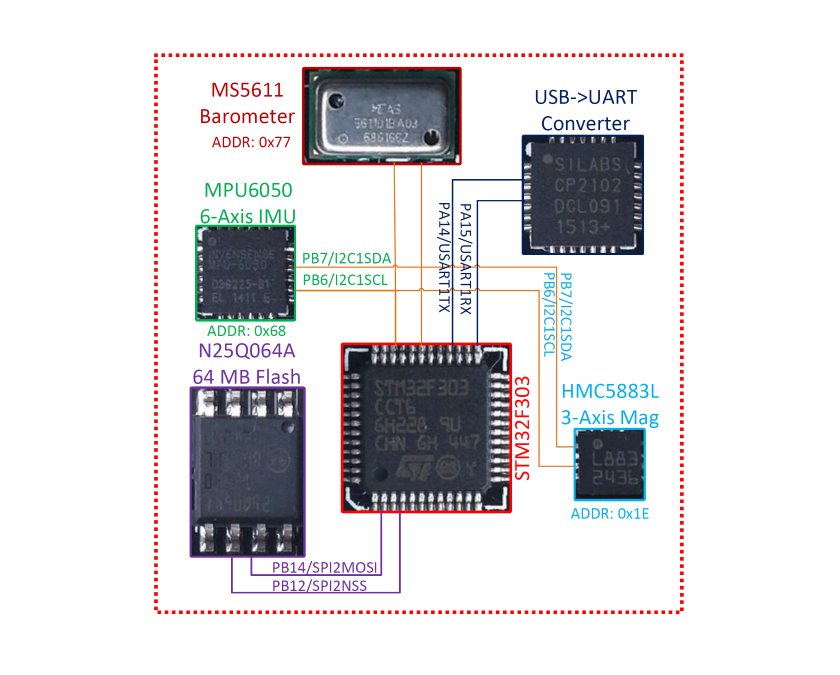
\includegraphics[width=0.95\textwidth]{figs/f3-deluxe-board}
\caption{F3 Deluxe on-board connections}
\label{fig:f3-deluxe-board}
\end{subfigure}
\caption{SPRacing F3 deluxe layout}
\label{fig:f3-deluxe-layout}
\vspace{-10pt}
\end{figure}
The embedded system is constructed around an ARM STM32F303\cite{stm32f303} based microcontroller. The micro-processor board is a commercial flight control board, specifically an SPRacing F3 Deluxe\cite{spracing}. CleanFlight or BetaFlight opensource software (from \cite{cleanflight} and \cite{betaflight} respectively) are typically used for this SPRacing F3 board; but despite open-source software its hardware specifications are  however not openly available. The reverse engineered electrical schematic for the board is included in App:\ref{app:deluxe-diagram} but a simplified overview of its internal connections is shown in Fig:\ref{fig:f3-deluxe-board}.
\par
The flight-controller has the following onboard peripherals; an I2C MPU-6050 6-axis gyroscope and accelerometer \cite{mpu6050} with an I2C connected HMC5883 magnetometer compass \cite{hmc5883}; an I2C MS5611 barometer \cite{ms5611} and finally 64 Mb of SPI flash memory. Consideration of sensor fusion effects of the above state-estimators is discussed subsequently in Sec:\ref{sec:simulation.state}. The caveats of Kalman filtering and discretized effects on the simulation loop are similarly discussed in that particular section.
\begin{figure}[hbtp]
\centering
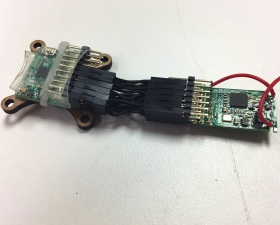
\includegraphics[width=0.55\textwidth]{figs/ppm-sbus}
\caption{SBUS converter \& 6CH receiver}
\label{fig:ppm-sbus}
\vspace{-20pt}
\end{figure}
\par
Two separate wireless communication loops are to be used. First; the system relays full state information for a complete 6-DOF X-Y-Z position and $\phi-\theta-\psi$~orientation autopilot system. Sent from an independent ground control station (\emph{GCS}) using 2.4 GHz XBEE S1 module(s)\cite{xbees1} which is connected to the flight controller via USART. Full state-estimation, using a multi-camera system (\cite{arnold}), and basic trajectory generation is performed on the GCS for the vehicle to track that trajectory. 
\par
Secondly; a partial trajectory (basic orientation) augmented pilot control input system, fail safe and secondary to the autopilot loop, is transmitted through a six channel 2.4 GHz radio frequency module. The secondary system allows for phsyical control without the need of a trajectory generation loop. The six CH received signals, otherwise permeated as six individual 20 kHz PWM signals via an OrangeRx R615x receiver \cite{r615x}, are encoded into a single proprietary S.BUS data stream (Fig:\ref{fig:ppm-sbus}). 
\par
The need for a serial bus (S.BUS) encoder, specifically using \cite{sbusencoder}, comes about as a consequence of the introduction of the eight additional servos. As a result, there are no longer six free additional timer input/output channels which can be dedicated to input capture of those RC channels. Encoding the received data to a serial data line means the six CH commands can be processed with a single RX channel by the microcontroller. The encoder implements a USART derivative communications standard called S.BUS. Shown in Fig:\ref{fig:sbus} the S.BUS data, captured with a logic analyzer \cite{saleae}, was used to ascertain the data stream's following parameters:
\par
\begin{tabularx}{\textwidth}{X X}
\begin{minipage}{\textwidth}
\begin{itemize}[itemsep=0em]
\item 25 Bytes per packet
\item 8-Bit byte length
\item 1 Start byte 0x240
\item 1 Byte of state flags
\item 1 Stop byte 0x0
\item Bytes are:
\vspace{-5pt}
\begin{itemize}[itemsep=0em]
\item MSB First
\item 1 start \& 2 stop bits
\item Even parity bit
\item Inverted
\item 100000 baud (b.s$^{-1}$)
\end{itemize}
\vspace{-5pt}
\end{itemize}
\end{minipage}
&
\begin{minipage}{\textwidth}
\begin{itemize}[itemsep=0em]
\item 22 total bytes of CH data 
\item Each channel's data is 11 bits long
\item 16CH encoded
\item Channel data is little endian prioritized
\item 14 ms idle time between packets
\item Packets are arranged:
\end{itemize}
{
$\overbrace{[0x240]}^{Start~byte}\overbrace{[8B_1][3B_2}^{CH1}|\overbrace{5B_2][6B_3}^{CH2}|\overbrace{2B_3][8B_4][1B_5}^{CH3}|\ldots$
\\
$\overbrace{7B_5][4B_6|}^{CH4}\ldots\longrightarrow\ldots\overbrace{3B_22][8B_23]}^{CH16}\overbrace{[8B_24]}^{Flags}\overbrace{[0x00]}^{Stop~byte}$
}
\end{minipage}
\\
\end{tabularx}
\begin{figure}[hbtp]
\centering
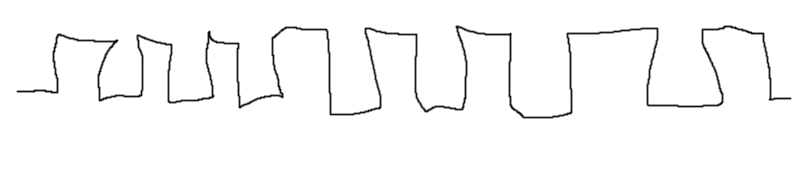
\includegraphics[width=\textwidth]{figs/sbus}
\caption{S.BUS data stream}
\label{fig:sbus}
\vspace{-10pt}
\end{figure}
\par
{\color{red}
The received information from the transmitted six channels is smoothed with a digital filter, using an infinite impulse response moving average filter. The filters difference equation can be as follows: 
\begin{equation}
y_n = \big(1-\frac{1}{N}\big)y_{n-1}+\frac{1}{N}x_n
\end{equation}
Moving over an average of $N=5$ samples which, each with a propagation delay of 14 ms due to S.BUS transmission, the filtered input channels have a 70 ms zero order holding time. The signal's sampling delays are sufficiently faster than the transfer times of the signals to not be consequence.
\par
Similarly all the measured RPM signals measured by the OrangeRx RPM speed sensors are filtered over five samples as well. Any received signals referred to are all post filtration. Filtering for state estimation made without using the inertial-measurement unit (using the camera system) is to be performed separately on the Ground Control Station computer.}
\par
Each of the eight digital servo actuators are controlled individually from $330~\text{Hz}$ center aligned PWM timer output compare channels (TIM2:CH1$\rightarrow$CH4 and TIM3:CH1$\rightarrow$CH4). Output pulses range from $1-2~\text{ms}$ to linearly control the rotational position. The servo's exact range and transfer function(s) is empirically determined next in Sec:\ref{subsec:proto.design.transfer}. The four $20~\text{A}$ brushless DC electronic speed controllers (\emph{ESC}s) are each driven from a $20~\text{Hz}$ PWM output (TIM4:CH1$\rightarrow$CH4), similarly with $1-2~\text{ms}$ input pulse widths. 
\par
There is a total of twelve PWM output compare signals drawn from the flight controller, eight for the servos and four for the ESCs. The servos are powered by a regulated $6~\text{V}$ DC $10~\text{A}$ power supply \cite{rotorstar} whilst the ESCs switch unregulated $14.1~\text{V}$ DC supplied from an external power tether. The DC supply could be drawn from a battery bank but that would adversely affect the weight of an already heavy platform.
\par
There is no integrated feedback for instantaneous RPM values available from the ESCs. Dedicated OrangeRX BLDC RPM sensors, \cite{orangerpm}, are used to measure each of the four motor's rotational speeds. Despite being termed \emph{brushless DC motors}, the motors are actually 3-phase motors which, when used with an ESC, behave like closed loop DC motors. The RPM sensors physically measure switching phases across two of the three motor phases, following that exact RPM can be ascertained. In general, the switching signal of a 3-Phase induction motor is shown by \cite{vfd} to be proportional to the rotational velocity:
\begin{equation}
F_{rps}=\frac{2\times F_{poles}}{\text{No. of rotor poles}}~~[\text{Hz}]
\end{equation}
The output signal generated by the OrangeRx RPM sensors varies the period of a 50\% duty cycle square wave, that wave frequency is directly proportional to the motor's pole switching frequency. The sensor output signal has a gain of 7 for the 14 pole BLDC Cobra motors. That gain is verified with the linear relationship(s) physically measured using an optical rotation sensor, plotted in Fig:\ref{fig:rpm-sensor}. Knowing exact RPM rates means the subsequent thrust and aerodynamic torques for the control plant inputs can be calculated with greater certainty.
\par
\begin{figure}[hbtp]
\begin{subfigure}{0.5\textwidth}
\centering
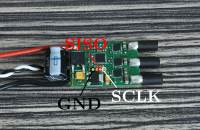
\includegraphics[width=0.98\textwidth]{figs/xrotor-20A}
\caption{XRotor 20A ESC connection guide\cite{xrotor}}
\label{fig:xrotor-20A}
\end{subfigure}
\begin{subfigure}{0.5\textwidth}
\centering
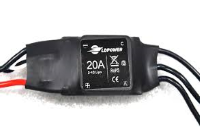
\includegraphics[width=0.98\textwidth]{figs/ldpower-20A}
\caption{LDPower 20A ESC with RPM sensor}
\label{fig:ldpower-20A}
\end{subfigure}
\caption{BLDC electronic speed controllers}
\vspace{-6pt}
\end{figure}
\par
The ESCs, although LDPower 20A devices, are re-flashed with BLHeli firmware \cite{BLHeli}. The LDPower ESCs (Fig:\ref{fig:ldpower-20A}) match Hobbywing Xrotor 20A ones (Fig:\ref{fig:xrotor-20A}) which both use SiLabs F396 microcontrollers; the same firmware can be flashed onto both MCUs. Custom BLHeli software provides greater refinement over configurations like the deflection range of inputs, but default values were used. The plot in Fig:\ref{fig:rpm-sensor-noload} shows the rotation per second, or otherwise frequency in Hz, speed curve for an unloaded motor; similarly in Fig:\ref{fig:rpm-sensor-prop} shows the speed curve when loaded for a $6\times 4.5$ prop. 
\begin{figure}[htbp]
\begin{subfigure}{0.5\textwidth}
\centering
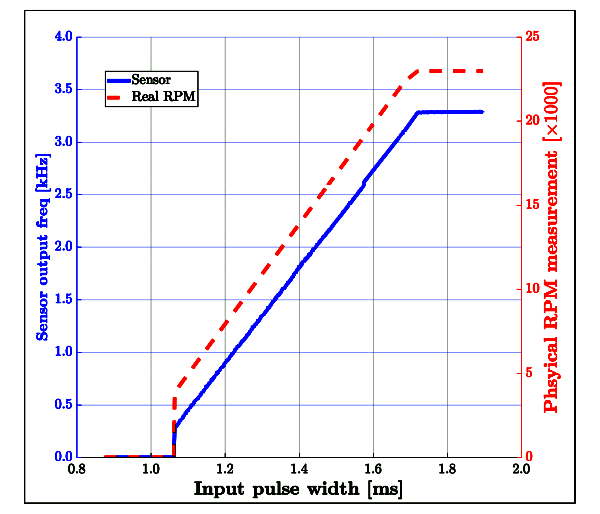
\includegraphics[width=\textwidth]{graphs/rpm-sensor-noload}
\caption{RPM sensor plot - no load}
\label{fig:rpm-sensor-noload}
\end{subfigure}
\begin{subfigure}{0.5\textwidth}
\centering
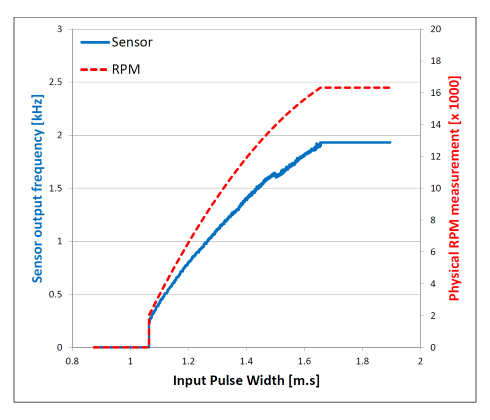
\includegraphics[width=\textwidth]{graphs/rpm-sensor-prop}
\caption{RPM sensor plot - 6X4.5 prop}
\label{fig:rpm-sensor-prop}
\end{subfigure}
\vspace{-4pt}
\caption{RPM sensor calibration plots}
\label{fig:rpm-sensor}
\vspace{-14pt}
\end{figure}
\par
The loaded speed plot for a BLDC motor with an attached prop in Fig:\ref{fig:rpm-sensor-prop} is slightly quadratic; that response is due to second order aerodynamic drag, quadratic with respect to the propeller's rotational speed (expanded on in Sec:\ref{subsec:dynamics.aero.bem}). Moreover, when the motor is torque loaded by the propeller, the ESC current limits rotational speeds at just over $16\times 10^3~\text{RPM}$.
\par
Timer channels are used to measure the varying frequency output from the RPM sensors. General purpose Timers 15 (TIM15:CH1$\rightarrow$CH2), 16 (TIM16:CH1) and 17 (TIM17:CH1) are configured to capture the input PWM signal generated by the speed sensors. Included on the I2C communication line is an I2C O-LED display for debugging and status update purposes.
\par
Any STM32 microcontroller is programmed through a dedicated debugging device. The ST-Link V2\cite{st-link} is the current proprietary device which, itself, is a specially programmed STM32F10 chip. The chip connects to the dedicated \textbf{S}erial \textbf{W}ire \textbf{D}ebugging ports of the target STM (\emph{SWD-CLK, SWD-IO} \& \emph{SWD-NRST}) and is interfaced via regular USBD+ and USBD- data lines. 
%====================================================
\subsection{Actuator Transfer Functions}
\label{subsec:proto.design.transfer}
%====================================================
\subsubsection*{Servo Transfer Functions}
%====================================================
\begin{figure}[htbp]
\centering
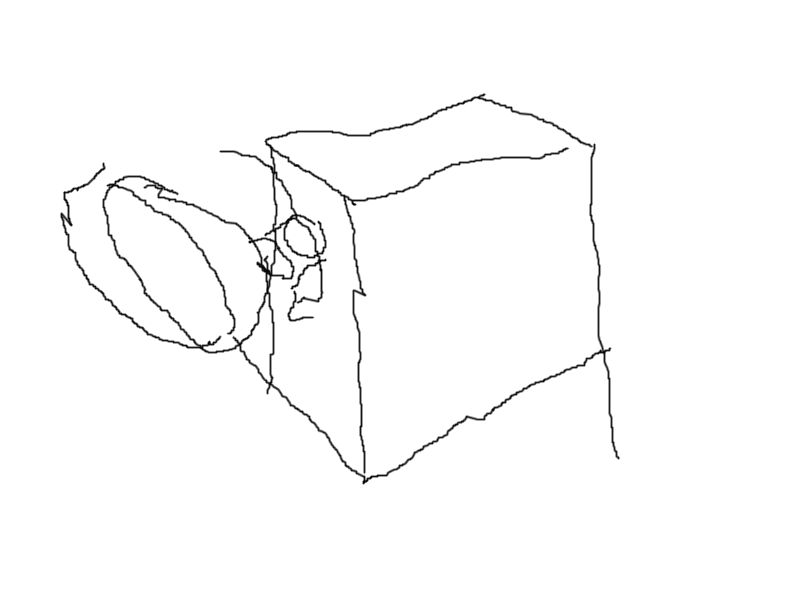
\includegraphics[width=0.68\textwidth]{figs/servo-position}
\vspace{-6pt}
\caption{Servo transfer function test rig}
\label{fig:servo-position}
%\vspace{-20pt}
\end{figure}
The range and step transfer functions of an unloaded servo were evaluated with the test rig illustrated in Fig:\ref{fig:servo-position}. The servo's output shaft was mechanically coupled to a rotatory potentiometer which was sampled to measure the shaft's rotational position. Full scale deflection for the digital servos are in fact greater than their quoted 180\textdegree ~range, each having an input range of around 230\textdegree ~(Fig:\ref{fig:servo-range}). The prototype control loop commands each servo position in open loop; the major loop controller gains designed in Sec:\ref{sec:simulation.tuning} are expected to account for minor loop actuator dynamics. However, the simulation must accurately represent the servo's transfer characteristics for such an assumption to hold true. 
\par
Considering the 180\textdegree ~servo limit was a design imposed constraint, one point of contention is the effect that such a constraint has on the feasible operating trajectories. The control algorithms derived in Ch:\ref{ch:control} are first tested with an ideal, continuous rotation servo actuator with similar rate limits and transfer characteristics. Following that servo limitations are introduced and the constraints to feasibly achievable trajectories are investigated in Sec:\ref{sec:simulation.saturation}.
\begin{figure}[htbp]
\centering
\begin{subfigure}{0.49\textwidth}
\centering
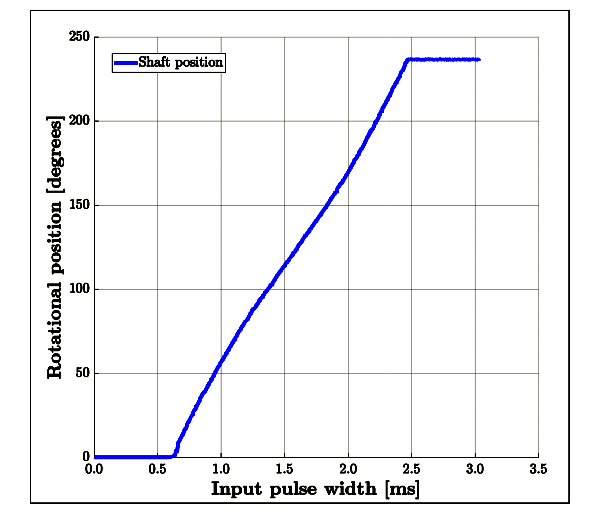
\includegraphics[width=\textwidth]{graphs/servo-range}
\caption{DS339-MG full Range}
\label{fig:servo-range}
\end{subfigure}
\begin{subfigure}{0.49\textwidth}
\centering
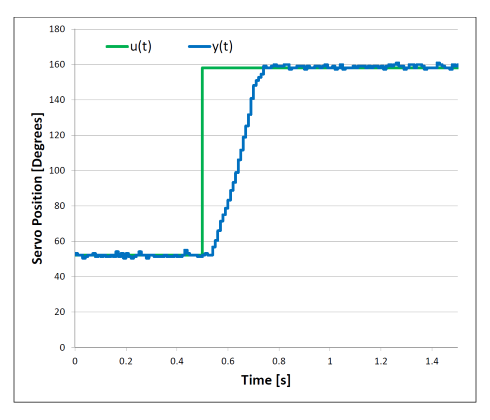
\includegraphics[width=\textwidth]{graphs/servo-step}
\caption{DS339-MG Step Response}
\label{fig:servo-step}
\end{subfigure}
\vspace{-8pt}
\caption{Unloaded servo transfer characteristics}
\label{fig:servo-no-load}
\vspace{-16pt}
\end{figure}
\par
For the servos whose rotational range and step response are shown in Fig:\ref{fig:servo-no-load}, the relationship between the input pulse-width $x~\text{m.s}$ and the rotational output position $y$ is given by:
\begin{equation}\label{eq:servo-range}
y(x)=
\begin{cases}\begin{array}{ll}
0\text{\textdegree} & ~~x<0.65~\text{ms}\\
129.12x-82.64 & ~~0.64~\text{ms} \leq x \leq 2.46~\text{ms}\\
230\text{\textdegree} & ~~x>2.46~\text{ms}\\
\end{array}
\end{cases}
\end{equation}\par
In practice the equation Eq:\ref{eq:servo-range} is changed such that 0\textdegree ~offset is taken at around a 50\% input, making its operational range $\pm 90$\textdegree . Each servo is mechanically rate limited to $60\text{\textdegree}/0.15~s$ or $400$ degrees per second with a dead time of $t_d\approx 1.2~\text{ms}$ and a (\emph{negligible}) mechanical deadband of $4~\mu\text{s}$. Each servo has an approximate (\emph{critically damped}) second order transfer function
\begin{subequations}\label{eq:servo-transfer}
\begin{equation}
G(s)_{servo}=e^{-t_d s}\frac{w_n^2}{s^2+2\zeta w_n s + w_n^2}
\end{equation}
\begin{equation}
=\frac{e^{-0.012s}(14.869)^2}{s^2+2(1)(14.869)s+(14.869)^2}
\end{equation}
With saturation limits from $|U(s)|$ for the PWM input magnitude:
\begin{equation}
Y(s)_{servo}=
\begin{cases}\begin{array}{ll}
0\text{\textdegree} & ~~|U(s)|<0.65\\
G(s) & 0.65 \leq |U(s)| \leq 2.46\\
230\text{\textdegree} & ~~|U(s)|>2.46\\
\end{array}
\end{cases}
\end{equation}
\end{subequations}
\par
The net transfer block for the servo is shown in Fig:\ref{fig:servo-block}, including saturating nonlinearities but neglecting the afore mentioned mechanical deadband\ldots
\begin{figure}[hbtp]
\centering
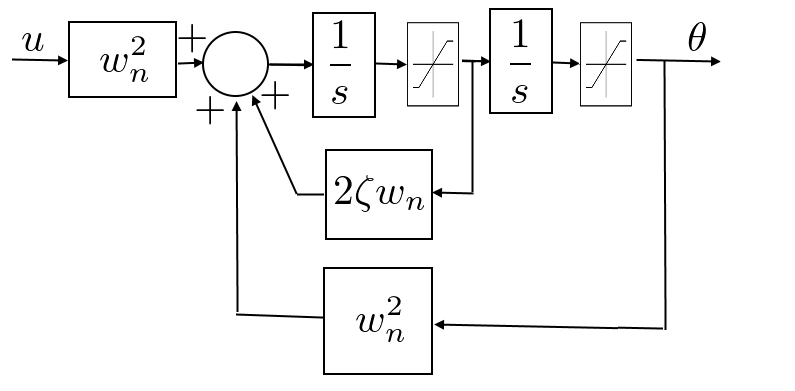
\includegraphics[width=0.8\textwidth]{figs/servo-block}
\vspace{-5pt}
\caption{Servo block diagram}
\label{fig:servo-block}
\vspace{-15pt}
\end{figure}
\par
The plot in Fig:\ref{fig:servo-step} shows the step response, at the \emph{shaft output}, of an unloaded servo. The servo's transfer characteristics when rotating the inner ring assembly (Fig:\ref{fig:inertia-inner}) are determined from the test rig in Fig:\ref{fig:servo-inner}. Fig:\ref{fig:servo-step-inner} shows the servo's step response {\color{Blue}$\mathbf{y(t)}$}, which is unchanged from Eq:\ref{eq:servo-transfer}, it then follows that for the inner ring's transfer function $\therefore G(s)_{inner}=G(s)_{servo}$. Even when actuating a loaded inner ring assembly with a propeller rotational velocity of 6500 RPM, plotted {\color{Red}$\mathbf{y'(t)}$}; the transfer characteristics are the same despite further increasing the torque load of the assembly due to the gyroscopic response, Eq:\ref{eq:prop-inertia}.
\begin{figure}[htbp]
\vspace{-6pt}
\centering
\begin{subfigure}{0.73\textwidth}
\centering
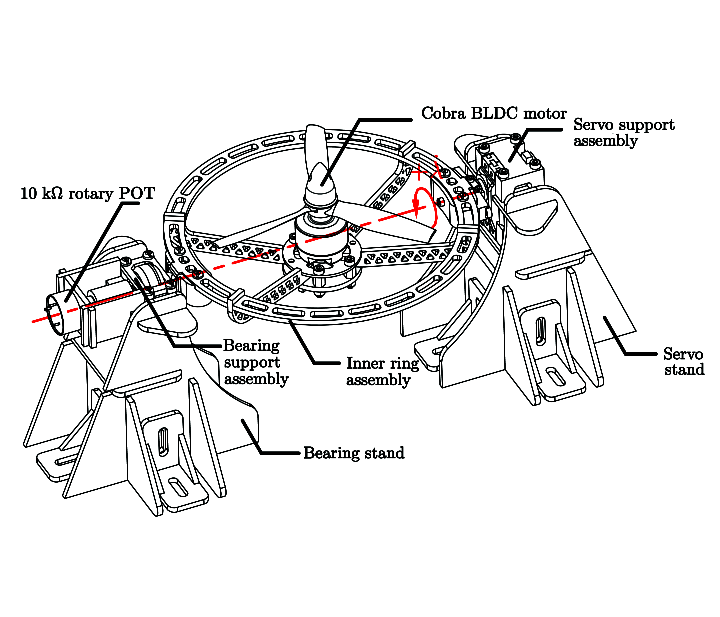
\includegraphics[width=\textwidth]{figs/servo-inner}
\vspace{-10pt}
\caption{Inner ring servo rig}
\label{fig:servo-inner}
\end{subfigure}
\par
\begin{subfigure}{0.49\textwidth}
\centering
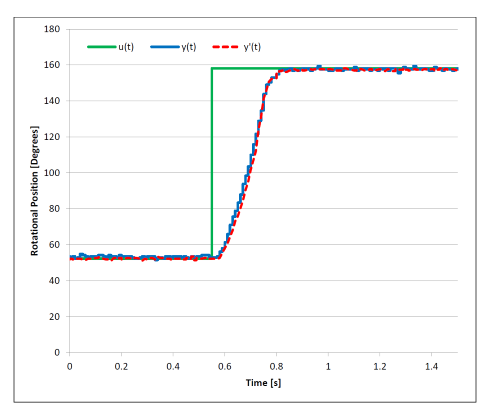
\includegraphics[width=\textwidth]{graphs/servo-step-inner}
\caption{Servo response plot}
\label{fig:servo-step-inner}
\end{subfigure}
\vspace{-4pt}
\caption{Inner ring servo characteristics}
\label{fig:servo-inner-character}
\vspace{-10pt}
\end{figure}
\par
Fig:\ref{fig:servo-step-middle} plots the step response for the servo actuating the middle ring assembly. Whilst its transients remain the same, oscillations are introduced at the settling point which demonstrates a second order under-damped plant. Those oscillations are as a result of the larger rotational inertia (Eq:\ref{eq:inertia.middle}) and flexure within the frame structure. It is important to specify that the oscillations are not at the servo's output shaft; the rotational position was measured with respect to the bearing supported shaft, coaxial to the servos (Fig:\ref{fig:servo-middle}). A separate, under-damped transfer fucnction is used for the middle ring's response, the rotational position $\alpha_i$ of the frame is to be used for thrust vectoring calculations in Eq:\ref{eq:motor-module-force-redirect}. Those harmonics are still present under load, plotted in {\color{Red}$\mathbf{y'(t)}$}, despite the frame being tensioned by the thrust. 
\begin{figure}[hbtp]
\vspace{-4pt}
\centering
\begin{subfigure}{0.88\textwidth}
\centering
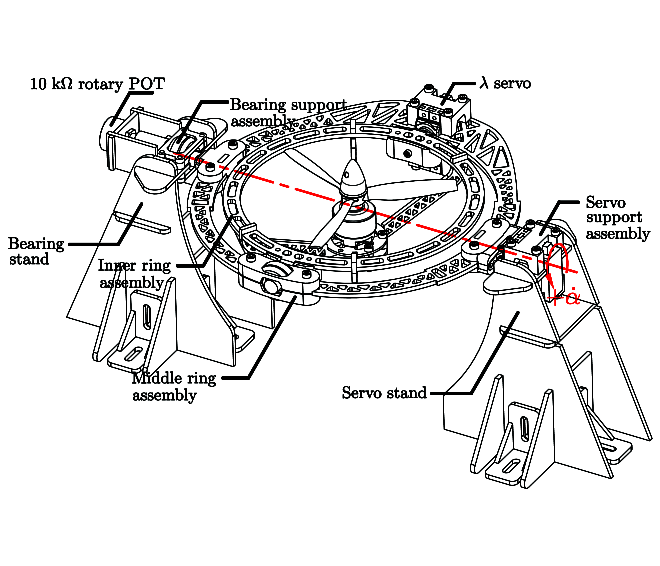
\includegraphics[width=\textwidth]{figs/servo-middle}
\vspace{-12pt}
\caption{Middle ring servo test rig}
\label{fig:servo-middle}
\end{subfigure}
\par
\begin{subfigure}{0.49\textwidth}
\centering
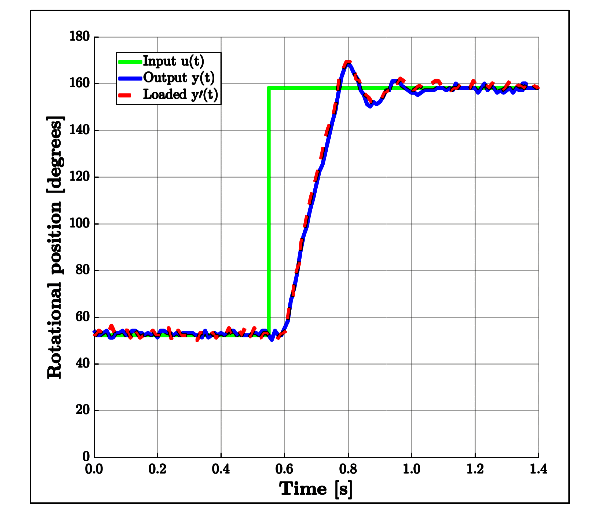
\includegraphics[width=\textwidth]{graphs/servo-step-middle}
\vspace{-10pt}
\caption{Servo response plot}
\label{fig:servo-step-middle}
\end{subfigure}
\vspace{-8pt}
\caption{Middle ring servo characteristics}
\label{fig:servo-middle-character}
\vspace{-18pt}
\end{figure}
\par
The mechanical structure could indeed be strengthened to reduce the oscillations present in Fig:\ref{fig:servo-middle}. Strengthening the frame would,however, increase the mass of an already weight constrained system. Instead the under-damped transfer function is included into the plant, that transfer function is:
\begin{equation}\label{eq:servo-transfer-middle}
G(s)_{middle}=\frac{e^{-0.012s}(12.591)^2}{s^2+2(0.454)(12.591)s+(12.591)^2}
\end{equation}
\subsubsection*{BLDC Transfer Functions}
Each Cobra 2208 BLDC motor, when loaded with a $6\times4.5$ propeller has a quadratic speed curve (plotted in Fig:\ref{fig:bldc-range}). This is as a result of the propeller's opposing aerodynamic drag, \emph{appromixately} proportional to the square of the propellers angular velocity (more on propeller aerodynamics in Sec:\ref{subsec:dynamics.aero.bem}).
\begin{figure}[htbp]
\centering
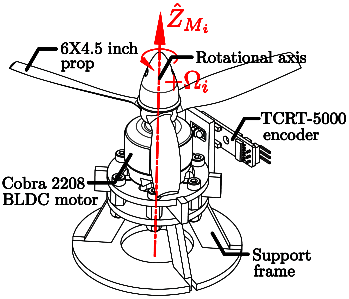
\includegraphics[width=0.48\textwidth]{figs/bldc-rpm}
\caption{BLDC rpm speed calibration and transfer function rig}
\label{fig:bldc-rpm}
\vspace{-16pt}
\end{figure}
\par
Using the BLHeli interface the input range for the motor's speed controllers can be adjusted, but for the purposes of this project, were left unchanged. That relationship between input pulse-widths to the ESC and output RPM sensor signal is given by the hybrid state equations for input range limits:
\begin{equation}
y(x)=
\begin{cases}\begin{array}{ll}
0 & ~~x<1.065~\text{ms}\\
-20593x^2 + 80187x - 60004 & ~~1.065~\text{ms} \leq x \leq 1.655~\text{ms}\\
16300 & ~~x>1.655~\text{ms}\\
\end{array}
\end{cases}
~~~\Bigg\}~~~~\text{RPM}
\label{eq:bldc-range}
\end{equation}
The upper limit in Eq:\ref{eq:bldc-range} and the motor's step response are both governed by the ESC's maximum current limit; in this case $20~\text{A}$. Imposing $10~\text{A}$ current limit, a potential consequence of using lower power ESCs, is plotted {\color{YellowGreen}$\mathbf{c(t)}$} in Fig:\ref{fig:bldc-step}. The current limit significantly restricts the motor's transient and steady-state performance. 
\begin{figure}[hbtp]
\begin{subfigure}{0.5\textwidth}
\centering
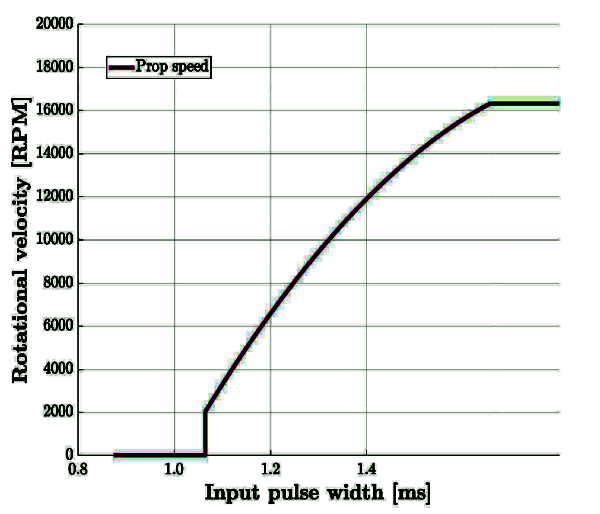
\includegraphics[width=0.98\textwidth]{graphs/bldc-range}
\caption{BLDC input RPM range}
\label{fig:bldc-range}
\end{subfigure}
\begin{subfigure}{0.5\textwidth}
\centering
\includegraphics[width=0.98\textwidth]{graphs/BLDC-step}
\caption{Cobra BLDC step response}
\label{fig:bldc-step}
\end{subfigure}
\caption{BLDC motor characteristics}
\end{figure}
\par
The motor's step response, {\color{Purple}$\mathbf{y(t)}$}, has a negligible dead time and 2\textsuperscript{nd} order dynamics, with a transient time constant far faster than the servo's plant. The motor's transfer function for speed in RPM is:
\begin{subequations}\label{eq:bldc-transfer}
\begin{equation}
G_{BLDC}(s)=\frac{1}{\big(1+1.7583s\times 10^{-3}\big)\big(1+1.7494s\times 10^{-3}\big)}~~~~[\text{RPM}]
\end{equation}
And saturation limits with input $|U(s)|$ for the PWM magnitude:
\begin{equation}
Y_{BLDC}(s)=
\begin{cases}\begin{array}{ll}
0\text & ~~|U(s)|<1.065\\
G(s) & 1.065 \leq |U(s)| \leq 1.655\\
16300 & ~~|U(s)|>1.655\\
\end{array}
\end{cases}
\end{equation}
\end{subequations}
\vspace{-22pt}
\par
The net transfer characteristics for a complete motor module then includes Eq:\ref{eq:servo-transfer} for $\lambda_i$ steps, Eq:\ref{eq:servo-transfer-middle} for changes in $\alpha_i$ and lastly Eq:\ref{eq:bldc-transfer} for changes in $\Omega_i$. A single module's transfer function is then bundled in the transfer block $C(s)$:
\begin{subequations}
\begin{equation}
u\cdot i = \begin{bmatrix}
\Omega_i(s)\\
\lambda_i(s)\\
\alpha_i(s)
\end{bmatrix}
= 
\begin{bmatrix*}[l]
B(s)_{BLDC}\\
N(s)_{inner}\\
M(s)_{middle}
\end{bmatrix*}
=C(s)
\end{equation}
And the actuator space for the $i^{\text{th}}$ motor module, $u\cdot i \in \mathbb{U}$, is limited by saturation conditions:
\begin{equation}
\mathbb{U}\cdot i \triangleq \begin{bmatrix*}[c]
0 : 16300\\
-90\text{\textdegree} :+90\text{\textdegree}\\
-90\text{\textdegree}:+90\text{\textdegree}
\end{bmatrix*}
\end{equation}
\end{subequations}
%====================================================
